\documentclass[conference]{IEEEtran}

\usepackage{times}

% numbers option provides compact numerical references in the text. 
\usepackage[numbers]{natbib}
\usepackage{multicol}
\usepackage[bookmarks=true]{hyperref}
\usepackage{graphicx}
\usepackage{amsmath}
\usepackage{amssymb}
\usepackage[capitalise]{cleveref}
\usepackage{xcolor}
\usepackage{algorithm}
\usepackage{algorithmic}
\usepackage{booktabs}
\usepackage{siunitx}
\sisetup{detect-weight=true,detect-family=true}

\newcommand{\red}[1]{\textcolor{red}{#1}}
\newcommand{\green}[1]{\textcolor{green}{#1}}
\newcommand{\blue}[1]{\textcolor{blue}{#1}}
\newcommand{\yellow}[1]{\textcolor{yellow}{#1}}
\newcommand{\command}{\mathbf{u}}
\newcommand{\state}{\mathbf{x}}
\newcommand{\commandt}{\mathbf{u}(t)}
\newcommand{\statet}{\mathbf{x}(t)}
\newcommand{\commandupdate}{\mathbf{\Delta u}(t)}
\newcommand{\stateerror}{\mathbf{\tilde{x}}(t)}
\newcommand{\model}{\mathcal{M}}
\newcommand{\invmodel}{\mathcal{M}^{-1}}
\newcommand{\ropeone}{\texttt{rope 1}}

\pdfinfo{
   /Author (Krishna Suresh, Chris Atkeson)
   /Title  (Learning Deformable Object Manipulation Using Task-Level Iterative Learning Control)
   /CreationDate (D:20101201120000)
   /Subject (Robots)
   /Keywords (Robot Learning;Imitation Learning;Robot Learning)
}

\begin{document}

% paper title
\title{Learning Deformable Object Manipulation Using Task-Level Iterative Learning Control}

% You will get a Paper-ID when submitting a pdf file to the conference system
\author{Krishna Suresh and Chris Atkeson\\
	Carnegie Mellon University\\
	Email: \texttt{{ksuresh2,cga}@andrew.cmu.edu}\\
\url{https://flying-knots.github.io}
}

% \newcommand{\shrink}{\def\baselinestretch{0.95}\large\normalsize} % <0.95 makes it ugly!!
% \shrink

\maketitle

\begin{abstract}
   Dynamic manipulation of deformable objects is challenging for humans and robots because they have infinite degrees of freedom and exhibit underactuated dynamics.
   We introduce a Task-Level Iterative Learning Control method for dynamic manipulation of deformable objects. We demonstrate this method on a non-planar rope manipulation task called the flying knot. Using a single human demonstration and a simplified rope model, the method learns directly on hardware without reliance on large amounts of demonstration data or massive amounts of simulation. At each iteration, the algorithm constructs a local inverse model of the robot and rope by solving a quadratic program to propagate task-space errors into action updates. We evaluate performance across 7 different kinds of ropes, including chain, latex surgical tubing, and braided and twisted ropes, ranging in thicknesses of 7--25mm and densities of 0.013--0.5 kg/m. Learning achieves a 100\% success rate within 10 trials on all ropes. Furthermore, the method can successfully transfer between most rope types in approximately 2--5 trials. \url{https://flying-knots.github.io}
\end{abstract}

\IEEEpeerreviewmaketitle

\section{Introduction}
% Dynamic manipulation of deformable objects is a challenging domain for both robots and humans. Deformable objects such as ropes and cloth are infinite degrees of freedom systems, highly underactuated, and lack accurate models. Expert humans can perform complex skills with deformable objects through practice and attention to key aspects of the task. Furthermore, humans leverage mental models of theses complex systems to inform their updates and efficiently improve their performance.
Dynamic manipulation of deformable objects is a challenging domain for both robots and humans. Deformable objects such as ropes and cloth have many unactuated degrees of freedom, and are expensive to model accurately.
% are infinite degrees of freedom systems, highly underactuated, and lack accurate models. 
We enable a robot to learn the dynamic task of tying a \textit{flying knot} as seen in \cref{fig:flying_knot}. This task is performed on a rope by executing a one-handed upward and twisting motion to form a loop and then arcing to strike near the end of the rope to flip it into the loop and completing a knot (\cref{fig:flying_knot}).

We adapt Iterative Learning Control (ILC) to improve a command trajectory through real-world trials. ILC is a powerful tool for enabling a robot to improve its performance on hardware, as introduced by \citet{arimoto_bettering_1984}, but we find that typical ILC formulations fail in deformable-object manipulation. 
ILC uses an approximate system model to convert task errors from real trials into command corrections; however, when ILC is learning to track rope target motions, equal weighting of task errors causes learning to fail. 

% inaccuracies in the system model limit the efficiency of ILC.

% errors may persist because: 

We leverage the underutilized Task-Level ILC \cite{12245} with two key features to enable success on deformable objects:
\begin{itemize}
  \item \textbf{Critical point objective:} 
  Instead of weighting trajectory errors equally throughout the task, we focus the robot's attention on the error in achieving a single rope configuration in the trajectory. This improves learning performance and enables the transfer of the task across large parameter variations. 
   \item \textbf{Task-level learning:} Our approach corrects the trajectory
   of state variables of the manipulated object, which
   goes beyond the usual ILC approach of correcting the
   robot trajectory.
\end{itemize}

We demonstrate the effectiveness of Task-Level ILC for deformable object manipulation. We show that learning is adaptable to variations in rope dynamics, demonstration types, and the system model. Overall, the key contributions of this work include the following:
\begin{itemize}
\item We explore Task-Level ILC for
deformable object manipulation, demonstrating that learning typically requires a small number of trials ($<10$ trials) and transfer
across different manipulated objects.
\item We develop a new approach to ILC for robots, which focuses attention
on \textit{critical points} of the error history.
\end{itemize}

% Move to related work
% Other interesting work such as \citet{chi_iterative_2022} and \citet{zhang_robots_2024} leverage open-loop commands for dynamic rope manipulation and demonstrate the effectiveness of optimization of a commanded trajectory and illustrate that errors in the task performance are repeatable.


\begin{figure}
    \centering
    \includegraphics[width=\linewidth]{figs/flying_knot_seq.png}
    \vspace{-4mm}
    \caption{Stages of a flying knot by both a human and a robot over 0.56s}
    \vspace{-5mm}
    \label{fig:flying_knot}
\end{figure}
\section{The Flying Knot Task}
% We are interested in deformable object manipulation,
% where the degrees of freedom of the deformable object
% are not fully actuated.
For this case study, we considered a variety of one
dimensional object manipulations, including
whipping, lassoing, throwing a rope to a target, fly casting, and attaching a rope to a distant object, such as a cleat or
tree branch by manipulating one end.
The flying knot task was chosen because it is impressive
but achievable by humans and fast robots.

There are several types of flying knots. We focus on the \textit{Overhand Knot}, in which one hand manipulates the end of a rope to tie an overhand knot, without changing the grip. As seen in \cref{fig:flying_knot}, the flying knot consists of multiple stages. The rope starts hanging from the hand. The hand is moved upward and twisted to form a loop. The rope collides with itself, and the end of the rope is flipped through the loop. The knot tightens as the rope falls. Often, a weight is added to the end of the rope.

\subsection{Flying Knot Objective}
\label{sec:flyobj}
While a successful flying knot is a well-defined task, the measure of whether a failed attempt is closer or further away from success is unclear. There are many key moments in the execution of a flying knot: loop creation, rope shape at collision, rope end passing through the loop, etc. In instructional materials for the flying knot, instructors often refer to the \textit{strike point} as a crucial step, as seen in \cref{fig:demos}. At least one rope self-collision occurs about halfway through task execution. While this moment in flying knot execution is not an exact predictor of task success, correctly matching this shape will likely lead to a knot. 

% An additional reason for choosing this metric is that we record the trajectory of markers on the rope up to the collision, since marker tracking typically fails at that point. 
We refer to this point in the rope motion as a \textit{critical point}. We provide the robot with a single demonstration of the flying knot for an example of the rope state at the \textit{critical point}. The flying knot task can be performed in several ways. The variations in demonstration share the same qualitative topological contact event, as visualized in \cref{fig:demos}, allowing the use of a single type of \textit{critical point} for learning.

\begin{figure}
    \centering
    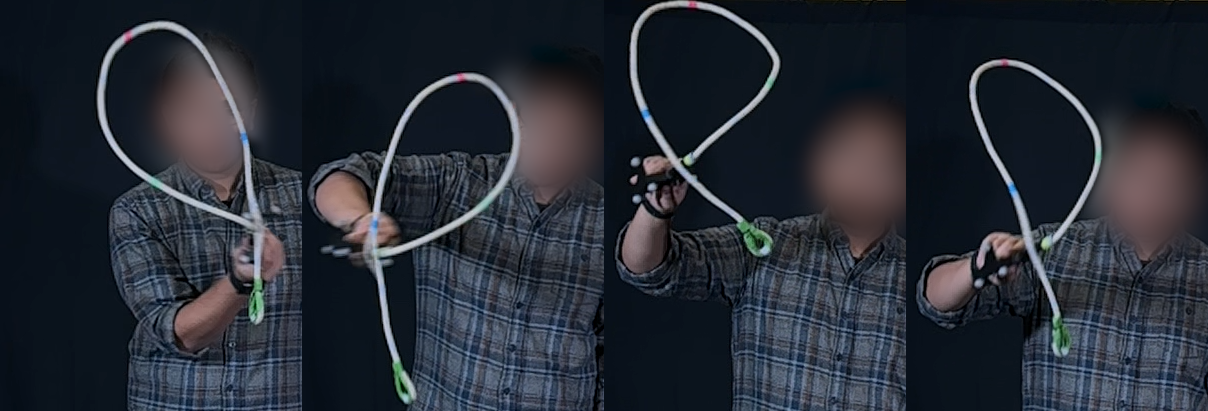
\includegraphics[width=\linewidth]{figs/demosvari2.png}
    \vspace{-5mm}
    \caption{\textbf{Critical point} for the flying knot across 4 demonstration variations. The shape of the rope at collision is used for the learning objective. }
    \label{fig:demos}
    \vspace{-5mm}
\end{figure}

\section{Related Work}
\subsection{Iterative Learning Control}
Iterative learning control is a command-update algorithm in which the system iteratively executes a feed-forward command in the real world and maps task errors into feed-forward command corrections. 
% Dynamics models can be insufficient for computing an acceptable command on the first try, so 
ILC leverages a system's repeatability to accumulate corrections across trials. Model-based ILC maps task errors to command updates with an \textit{inverse model} \cite{an_model-based_1988}. 

\textbf{Classical Iterative Learning Control (ILC)} studies how to improve performance on tasks that repeat over trials by updating a feedforward command based on errors. Early work formalized the idea of ``bettering'' robot operation via iterative error-based updates \citep{arimoto_bettering_1984}. In robotics, ILC-style trajectory learning through practice was demonstrated on manipulators using explicit (possibly imperfect) linear models and approximate inversion \citep{atkeson_robot_1986,an_model-based_1988}, and subsequent work analyzed convergence and design choices for robot manipulators and other repetitive systems \citep{kuc_iterative_1991,moore_iterative_1992}.

\textbf{Optimization-based ILC} or Norm-Optimal ILC formulations showed how to incorporate constraints and compute command corrections via an optimization objective. \citet{schoellig_optimization-based_2012} demonstrated aggressive quadrotor trajectory tracking by leveraging convex programs to reduce errors, and \citet{4020374} applies norm-optimal methods for real-time control of industrial gantry robots.

% by solving convex programs for aggressive quadrotor trajectory tracking  \citep{schollig_optimization-based_2009}.  applies optimization-based methods for tracking at a subset of task points \cite{6200836}.

% \textbf{Optimization-based ILC} formulations showed how to incorporate constraints and prior model structure by solving convex programs \citep{schollig_optimization-based_2009}. These ideas were later extended to aggressive trajectory tracking in aerial robots via quadratic programs and model-based filtering, demonstrating that accurate tracking can be achieved despite significant unmodeled dynamics \citep{schoellig_optimization-based_2012}. 


\textbf{Event-based ILC methods} focus learning on a subset of the task, such as the terminal states\cite{chi2015adaptive}, point-to-point \cite{8013126}, time windows \cite{1384669}, and event triggers \cite{lin2020event}. In general, placing learning attention at key moments of the task has worked in many domains, including non-robotics industrial domains such as CNC machine tools, wafer-stage motion systems, injection molding, induction motor drives, automotive braking/vehicle control, rapid thermal processing, and semi-batch chemical reactors \cite{1636313}.


\textbf{Modern learning methods} have recently been combined with ILC: using approximate simulators to propose local policy improvements \citep{abbeel_using_2006}, framing ILC through regret minimization \citep{agarwal_regret_2021}, and explaining when ILC can outperform planning with a misspecified model \citep{vemula_effectiveness_2022}. Additional work introduces ILC-style model-gradient updates in deep off-policy reinforcement learning to improve sample efficiency \citep{gurumurthy_deep_2023}. 

In our work, we leverage optimization-based and event-based techniques to attend learning to the \textit{critical points} of the task.

% \subsection{Task-Level Learning}
% \textbf{Task-level learning} 
% \subsection{Task-Level Iterative Learning Control}
% \begin{itemize}
%    \item - Echo cancelling, zoom call updates impulse response. this is kinda ILC if impuse response is lookup table. Another similar thing is maternal heart beat detection.
% - 60Hz RF adds interference to neuro measuring
% - Signal processing applications
% - any robot doing music
% - maybe the robot painting stuff from peter
% - factory robots ILC, welding quality: https://ieeexplore.ieee.org/document/7799380
% - https://ieeexplore.ieee.org/document/4587211
% \end{itemize}

\subsection{Deformable Object Manipulation}
\textbf{Quasi-static deformable object manipulation}, such as the handling of rope, cable, and cloth, has been addressed in a number of works \cite{9813374, doi:10.1126/scirobotics.abd8803} where many approaches focus on domains with strong perception and geometric priors \citep{tang_framework_2018} and imitation/representation learning for rope manipulation \cite{nair2017combining,hannus2024dynamic,huang2023act}. 

\textbf{Dynamic deformable object manipulation} focuses on faster tasks, such as whipping \cite{nah_2020}, cloth flinging \cite{chen_efficiently_2022, 5979606}, and dynamic rope knotting \citep{yamakawa_dynamic_2013}. 
% Iterative learning-based methods have also emerged for dynamic skills. 
Iterative Residual Policy proposes online action refinement via a learned residual dynamics model \citep{chi_iterative_2022}. Related works study learning for whip targeting, combining structured motion primitives with online adaptation or reinforcement learning \citep{xiong_online_2021,wang_learning-based_2024}.

Recent work has further explored dynamic cable and cloth behaviors with self-supervised data collection. Real2Sim2Real learning enables planar robot casting of cables by fitting simulators from physical rollouts \citep{lim_real2sim2real_2022}, and subsequent systems learn to dynamically manipulate fixed-endpoint cables via arcing motions \citep{zhang_robots_2024} or free-end cables in planar settings \citep{wang_self-supervised_2024}. 

In \citet{ha2021flingbotunreasonableeffectivenessdynamic}, \citet{chi_iterative_2022}, and \citet{zhang_robots_2024}, system models are learned with large-scale simulated data, but our use of Model-Based ILC eliminates the need for large-scale simulated data collection. 

In these works, commands are executed as feed-forward trajectories and demonstrate the repeatability of dynamic deformable object manipulation. Similarly, we leverage feedforward trajectories in the flying knot task.

\section{Method: Task-Level Iterative Learning Control}

\subsection{Iterative Learning Control}
Iterative Learning Control (ILC) is a data-efficient learning method for repetitive tasks. ILC maps task error trajectories $\stateerror$ to command trajectory updates $\commandupdate$ to iteratively refine a full sequence of commands. ILC can improve task performance beyond methods that generate commands solely from a system model, since it can correct for unmodeled dynamics. 
ILC is often applied to robot trajectory-tracking problems to minimize tracking errors caused by unmodeled system dynamics (e.g., friction, cogging torques, and gear backlash and play).

The command trajectory $\commandt$ that ILC corrects is a function of task phase (or time) rather than a control policy, which is a function of state. 
A time-dependent feedforward command has N parameters, where N is the number of samples. A feedback control policy typically has several orders of magnitude more
parameters.
% ($\text{number of resolutions} \times {\text{dimensionality}}$).
% for a lookup table.

Model-based ILC uses a system model $\model$ which maps commands to predictions of task performance. This system model may be inaccurate, but its gradient information accelerates learning, since knowledge of the command update direction need not be obtained from the real system. ILC inverts the system model, $\invmodel$, to map the real system's task errors into estimated command errors, which are subtracted from the current command. An overview of ILC is seen in \cref{fig:ilc_system}.
% ILC subtracts the predicted command errors from the current command at each iteration. 
If this system model is perfect, then all errors would be removed in one step. Even when the system model is inaccurate, if the command update direction (gradient) has a component in the required command update direction, command updates accumulate and iteratively reduce task errors. 


\subsection{Task-Level Iterative Learning Control}
ILC is often used for robot trajectory tracking. In trajectory tracking, the objective and the command are related by the robot dynamics, which are often modeled accurately. Trajectory-tracking ILC usually weights errors along the trajectory equally. 

In Task-Level ILC, task errors are similarly mapped to feed-forward robot command improvements. In this work, task errors are defined as deviations in the state variables of a deformable manipulated object. In addition, we explore the use of \textit{critical point} objectives, which focus on the error at \textit{critical points} along the trajectory.

% but focus on task errors at a single point along the trajectory (\textbf{critical point objective}) and on correcting errors in the state variables of the manipulated object (\textbf{task-level learning}). 

\begin{figure}
    \centering
    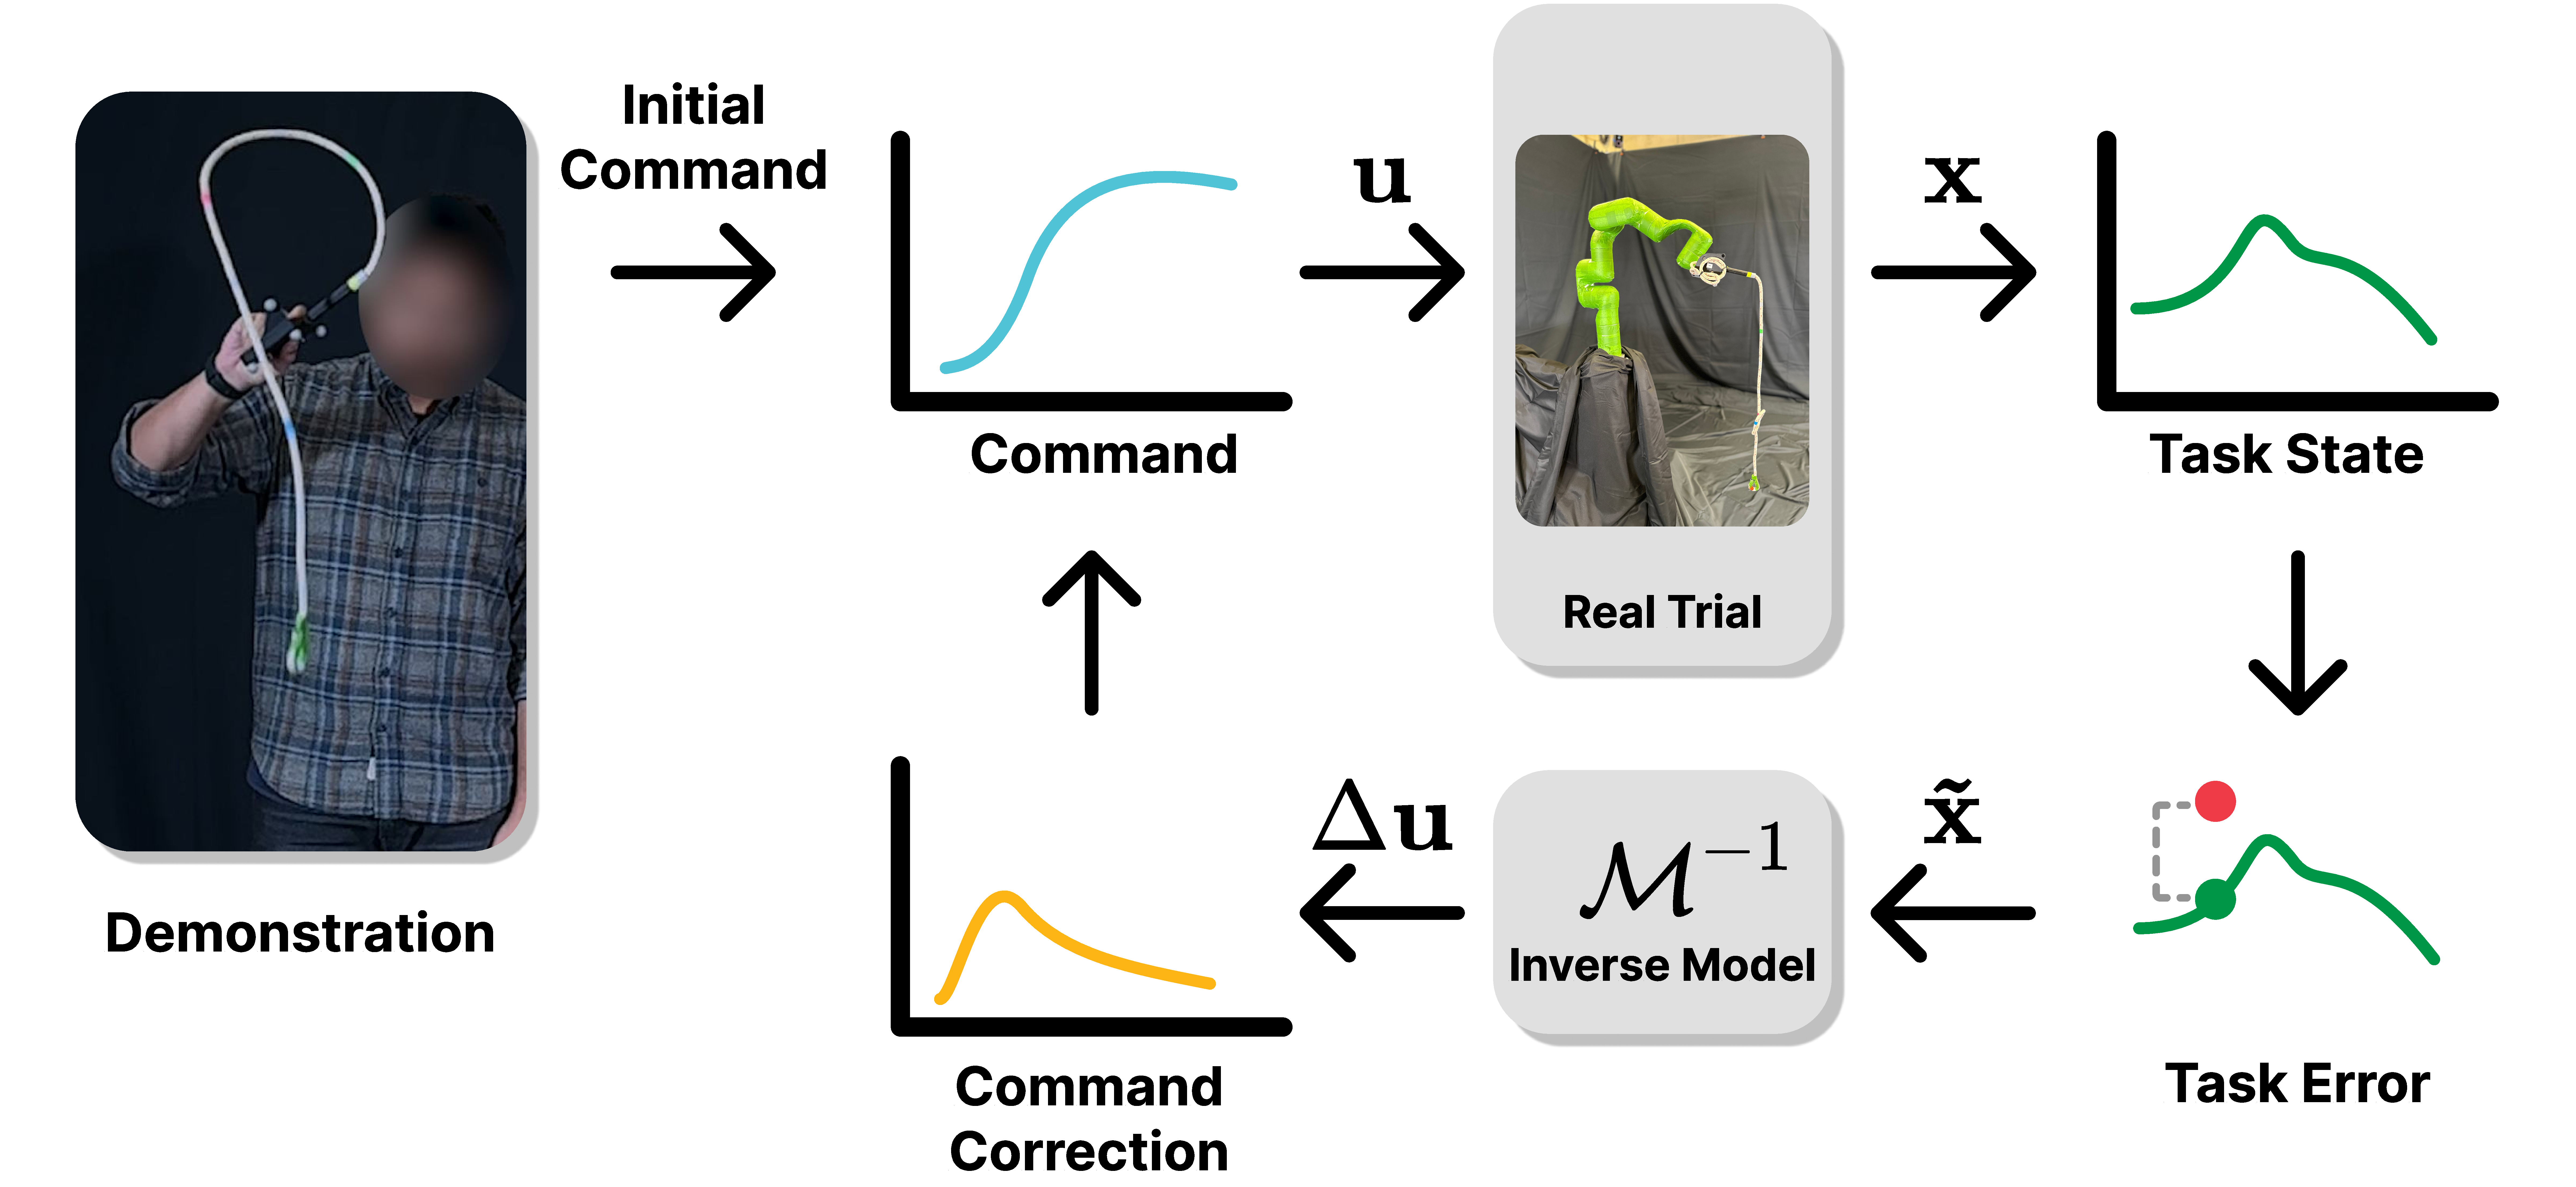
\includegraphics[width=\linewidth]{figs/ilc_system_figure.pdf}
    \vspace{-3mm}
    \caption{\textbf{Task-Level Iterative Learning Control System:} A demonstration is converted to an initial command. The command trajectory $\commandt$ is executed on the real system, and the resulting trajectory $\statet$ is measured. The task error $\stateerror$ at the \textit{critical point} is mapped through the inverse model $\invmodel$ to command trajectory corrections $\commandupdate$, which are applied to the current feedforward command, closing the learning loop.}
    \label{fig:ilc_system}
    % \vspace{-mm}
\end{figure}
% but allow for improvement of task performance external to the direct actuation of the system. In our setup, the rope is an unactuated high degree of freedom system which the robot can only control through motion of the hand. 

% Furthermore, we change the standard ILC setup to focus the attention of the learning to a single \textit{critical point} of the task rather than equally weighting the task errors. This improves learning performance and also enables transfer learning of the task to new ropes which may require different motions before the \textit{critical point}.  

\cref{alg:task_level_ilc} summarizes Task-Level ILC.
\begin{algorithm}
  \caption{Task-Level Iterative Learning Control (Task-Level ILC)}
  \label{alg:task_level_ilc}
  \begin{algorithmic}[1]
    \STATE \textbf{Inputs:} initial command $\command_{0}(t)$; reference critical-point state $\state^{\text{demo}}(t_c)$; \textit{critical point} $t_c$; inverse model $\invmodel$; $K$ iterations
    \FOR{$k = 0$ \TO $K$}
      \STATE $\state_{k}(t) \leftarrow \texttt{Trial}(\command_{k}(t))$ 
      \STATE Critical-point error $\tilde{\state}_{k}(t) \leftarrow \mathbf{x}_{k}(t_c) - \state^{\text{demo}}(t_c)$
      \STATE Command update $\Delta \command_{k}(t) \leftarrow \invmodel\!\left(\tilde{\state}_{k}(t)\right)$ %\hfill (e.g., solve inverse-model QP)
      \STATE Update $\command_{k+1}(t) \leftarrow \command_{k}(t) - \Delta \command_{k}(t)$
    \ENDFOR
  \end{algorithmic}
\end{algorithm}

\begin{figure*}[t]
  \centering
  \includegraphics[width=\textwidth]{figs/critvseq.png}
    \vspace{-4mm}
  \caption{\textbf{Critical point vs equal-weighted objective learned commands.} Each row is a real trial after 8 iterations with the corresponding objective. The green rope is the measured state from the real trial, and the red rope is the goal rope from the demonstration. The rope state at 0.46s is the \textit{critical point}. The \textit{critical point} objective trial results in a successful flying knot, while the equal-weighted objective trial results in a failure. }
  \label{fig:critvseq}

    \vspace{-3mm}
\end{figure*}
\subsection{Critical Point Objective}
\label{sec:critical_point}
The \textit{critical point} is defined as a key moment in the task at which all task error reduction is targeted. 
% Focusing on errors at a single point of the trajectory reduces the weight given to insignificant parts of the execution. 
For the flying knot task, we select the state of the rope at collision time $t_c$ in the demonstration as the \textit{critical point} as described in \cref{sec:flyobj}. 
% The \textit{critical point} was selected because it is the most discernible branching point in task success, is clearly defined, and is measurable. Placing the critical point at the collision simplifies the object, system model, and measurements. 
% The state of the rope at contact is also the last measurable state with our rope tracking system. 
Task-Level ILC attempts to generate a feed-forward trajectory before the collision to match the rope state of the demonstration only at the moment of collision. Therefore, rope-tracking errors before and after the \textit{critical point} are ignored as seen in \cref{fig:critvseq}

Eliminating task errors from the objective for times after contact also simplifies the modeling problem, as we only need to model free rope motion rather than the more complex contact physics between rope or finger and the end of the rope.
 
\subsection{Command Parameterization}
We parameterize the feed-forward robot command as 10 Bezier curves (7 joints + 3 base translation dimensions) with 8 knot points equally spaced in time: $\commandt \in \mathbb{R}^{10 \times 8}$. 
The base translation dimensions ensure translation invariance of the task objective, with constraints that prevent the robot base location from moving \cref{eq:base}. 
The fixed total execution time of the command $T$ is defined by the total length of the demonstration hand motion. 
Given $\commandt$ and $T$, a Bezier curve is computed using the Bezier function $\mathcal{B}$. This spline generation of the robot's
desired trajectory command is described in more detail in Appendix~\cref{sec:bezier}.
\subsection{Robot Model}
We model the robot as a kinematic chain parametrized by robot joint angles $q$. Because the robot's controller is driven by commanding
desired robot joint angles, any desired trajectory $\mathbf{q}_d(t)$ that satisfies the robot's joint position, velocity, and acceleration limits is trivially modeled with the robot motion matching the command, $q_d=q$. 
The desired trajectory is executed by the control system provided by the robot manufacturer, which mostly consists of joint-level PD servos.
Joint trajectories $\mathbf{q}(t)$ are mapped through the robot's forward kinematics $\mathcal{K}(\mathbf{q}(t))$ to determine the trajectory of the hand fingertip. 
While the real robot has more elements that can be modeled (e.g., link dynamics, actuation model), we find that this simple model is sufficient for ILC to improve the command. The robot model does not need to account for rope motion since the robot has joint actuators with a 100:1 gear ratio, so the rope's impact on the robot's dynamics is negligible.

% Our robot has joint actuators with a 100:1 gear ratio, so the rope's impact on the robot's dynamics is negligible. Therefore, the robot model does not need to account for the rope's motion. 
\subsection{Rope Model}
We model the rope as a 3D serial chain of point masses $m$ connected by fixed-distance constraints of length $l$. Each joint in the rope has a bending stiffness $k$ and a damping coefficient $b$. Since ropes are approximately self-similar, we use a single $m,k,b$ parameter for all but the last rope links and joints. The ropes we evaluate with have a weight attached to the end, which is approximated with a different end link mass $m_e$. Our approximate rope model has far fewer degrees of freedom than the true rope dynamics, with only $N=11$ links, which has proven adequate in this work. The unit scaling of these parameters is with respect to $m$, which we set to 1, resulting in only 5 model parameters ($k, b, m_e,l,N$).

The first point on the rope model is kinematically driven by the robot model's fingertip trajectory. We can define the rope dynamics model as a function $f$, which simulates the rope state given the initial rope configuration $\mathbf{z}_0$ and a position trajectory of the first link (full derivation found in Appendix~\cref{sec:dynamics_model}). This makes the overall system model, as seen in \cref{fig:system_model}, the following:
\begin{align}
   \model(\commandt, \mathbf{z}_0) = f(\mathcal{K}(\mathcal{B}(\commandt, T)), \mathbf{z}_0)=\hat\state(t) \label{eq:dynamics}
\end{align}
where $\hat \state$ is the model prediction of the rope state. To simulate the rope dynamics, we implement a maximal coordinate variational integrator dynamics model from \citet{lavalle_linear-time_2021}.

\begin{table}[t]
    \centering
    \caption{Rope Model Parameters}
    \label{tab:simulation_params}
    \begin{tabular}{l c}
        \hline
        \textbf{Parameter} & \textbf{Value} \\
        \hline
        Stiffness & $1\times10^{5}$ \\
        Damping & $50$ \\
        End Mass & $5$ \\
        Simulation Timestep & $0.005$ \\
        \# Links & $11$ \\
        Link Length & $0.1$m \\
        \hline
    \end{tabular}\\
    \vspace{3mm}
    {\small The unit scaling of stiffness, damping, and end mass is defined with respect to a link mass of 1.}
    \vspace{-3mm}
\end{table}
\begin{figure}
    \centering
    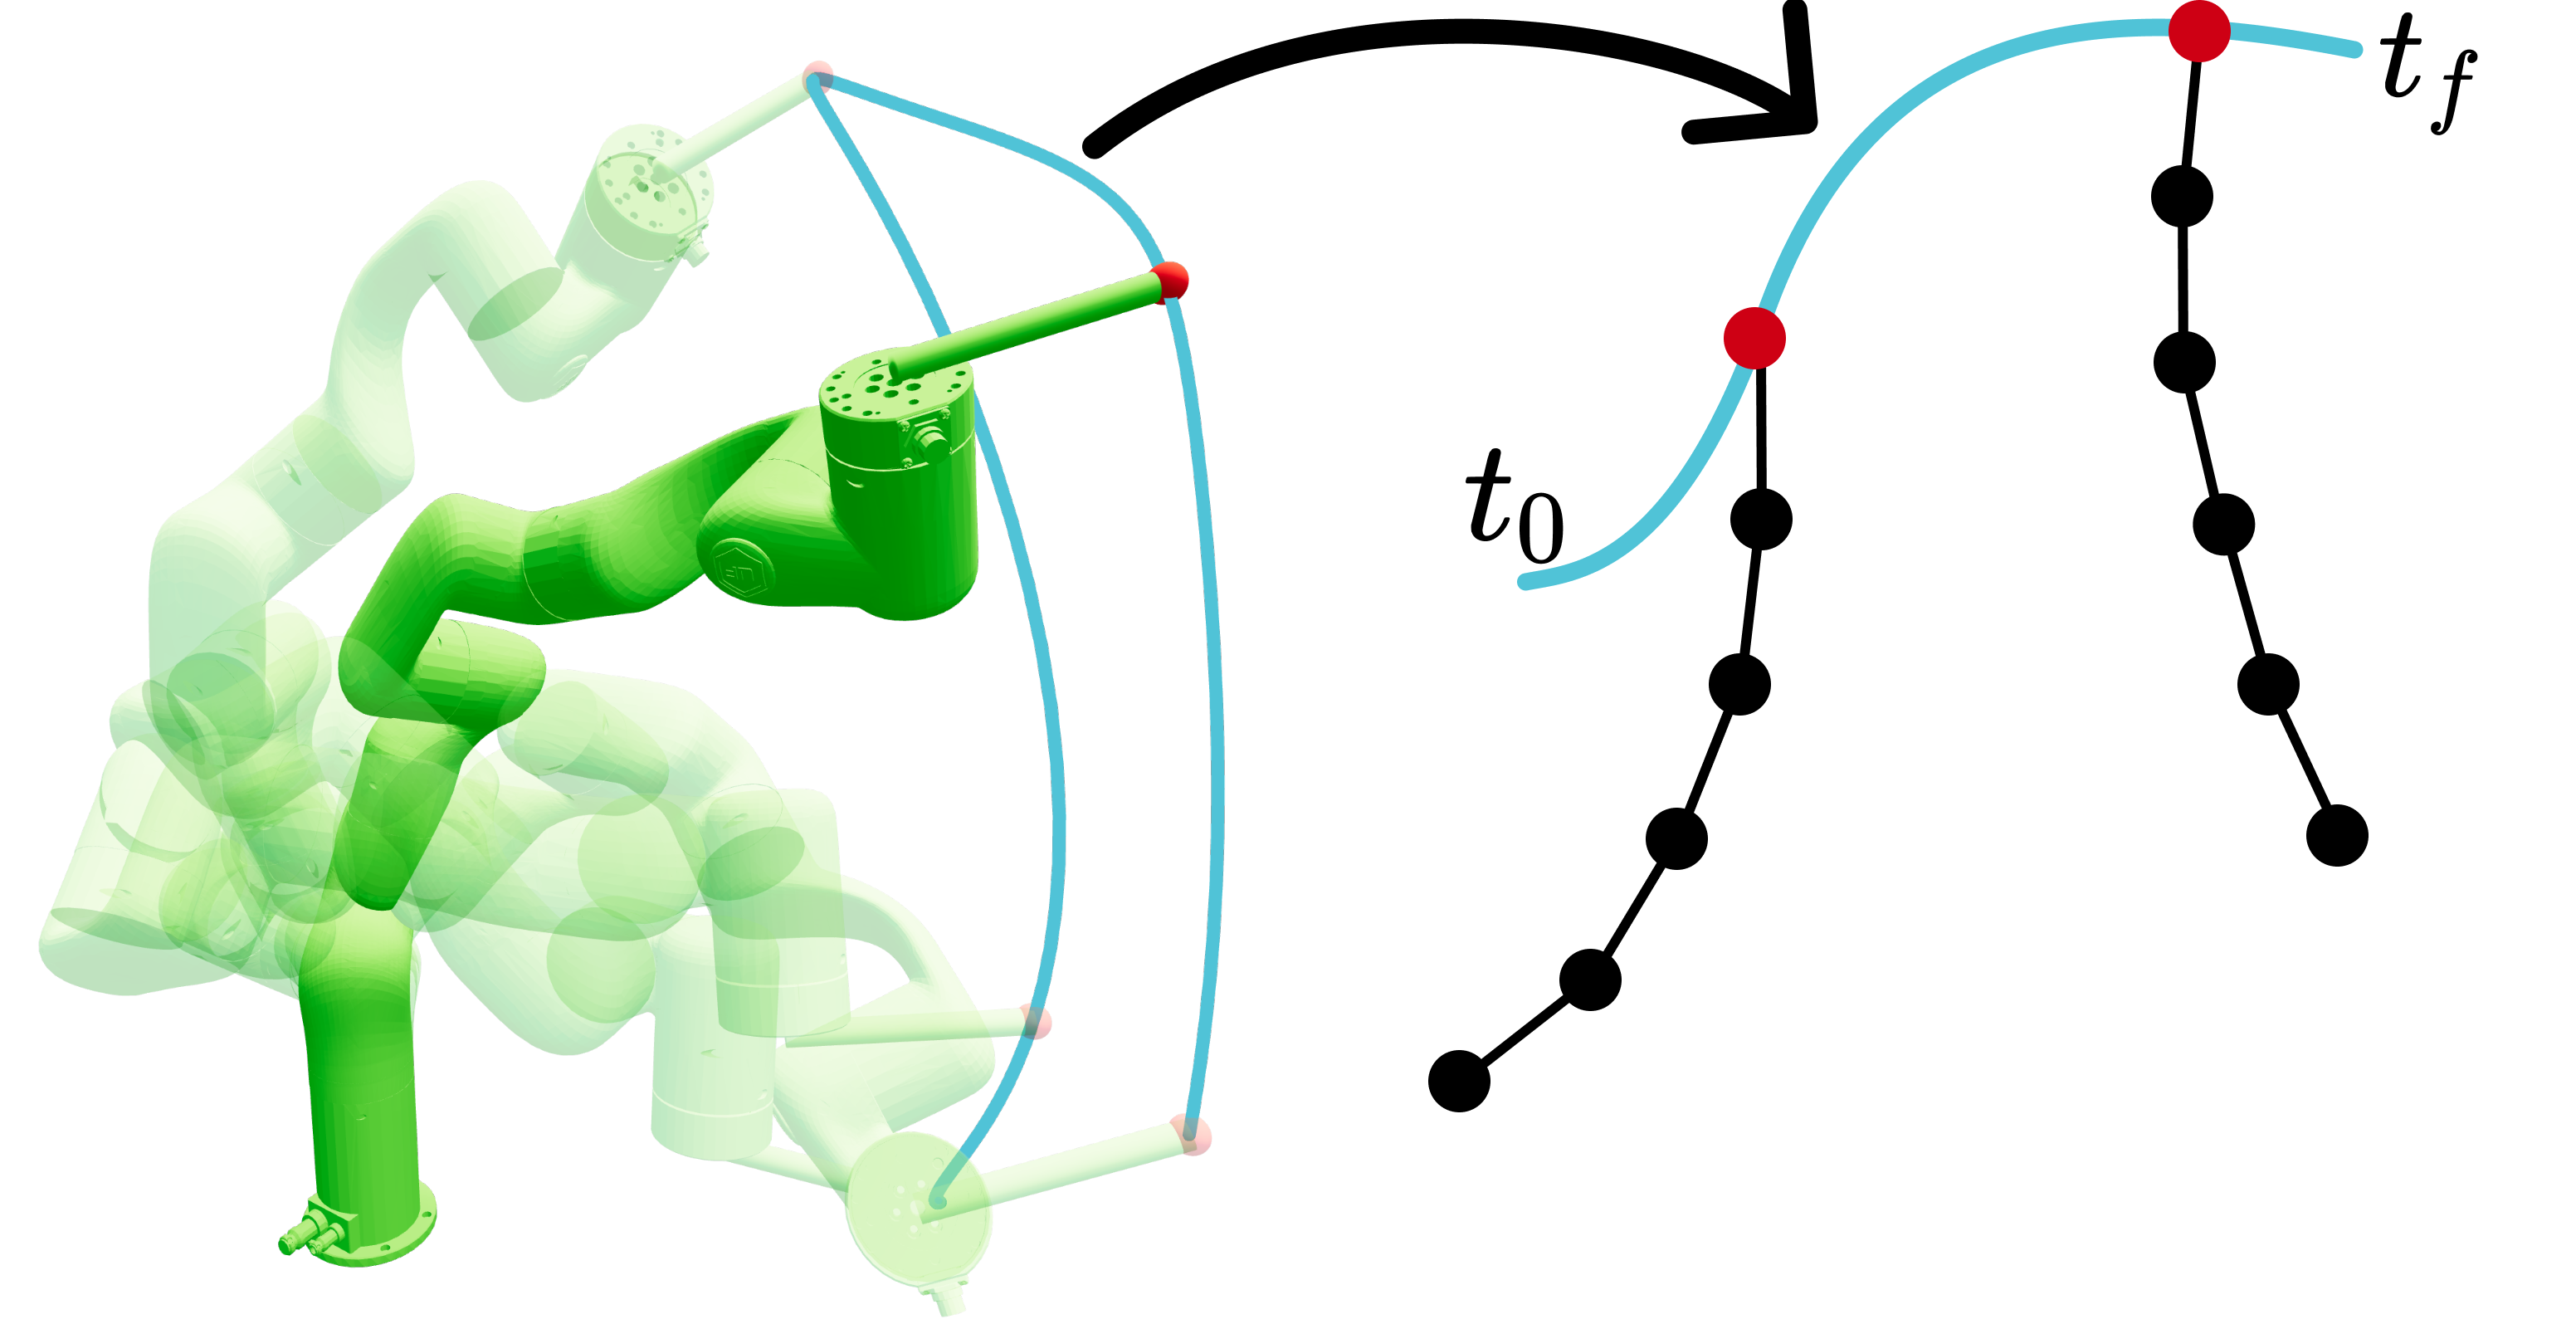
\includegraphics[width=\linewidth]{figs/system_model.png}
    \vspace{-3mm}
    \caption{\textbf{Left:} Kinematic robot model at various stages of a command. The opaque robot is at the point of contact. \textbf{Right:} Graphical representation of the point mass rope model. The robot's fingertip trajectory kinematically drives the first red dot. The remaining links are bound by distance constraints, and each joint has stiffness and damping. Together, the robot and rope models define our system dynamics model. All 3D visualization are created using Viser \cite{yi2025viser}.}
    \label{fig:system_model}
    \vspace{-5mm}
\end{figure}

\subsection{Optimization-Based Inverse Model}
Previous model-based ILC methods typically use an inverse model $\invmodel$ that equally weights all parts of the trajectory, which is well-suited for trajectory tracking but is insufficient for Task-Level ILC. Furthermore, task constraints such as robot joint dynamics limits are not typically handled by these inverse models. Methods for an optimization-based inverse model were introduced for trajectory tracking in \citet{schoellig_optimization-based_2012} and \citet{schollig_optimization-based_2009}. 
A Quadratic Program (QP) is formulated to minimize a quadratic task objective while satisfying linear constraints. The system model is imposed as a linearized dynamics constraint.

% Based on the measured robot motion, we simulate the rope dynamics, and then
% linearize the rope model M about the current rope trajectory
% How does the observation of the rope affect all this?
% Are you simulating the rope motion or measuring it?

% How does this get mapped down to x_squiggle, so
% M_inverse( x_squiggle - x_squiggle_desired ) can
% be computed?

Based on the measured robot motion, we simulate the rope dynamics and linearize the system model $\model$ about the current simulated rope trajectory $\hat\state_k(t)$ and current command $\command_k(t)$:
% To leverage this formulation, we simulate the true robot motion from the current command through the rope dynamics model $f$ and linearize the system model $\model$ about the current trial command $\command_k$ and model prediction $\hat\state_k$:
\begin{align}
   \mathbf{M} = \left.\frac{\partial \model}{\partial \commandt}\right|_{(\hat\state_k(t),\command_k(t))} \label{eq:dyn}
\end{align}

We define the quadratic optimization objective $\mathbf{Q}$ to be a state-error-tracking cost applied only at the \textit{critical point} $t_c$ of the demonstration. A control cost $\mathbf{R}$ penalizes updates to the 7 arm joints at each knot point for all $t$.

This formulation allows explicit inclusion of linear robot dynamics constraints $\mathbf{J}_p,\mathbf{J}_v,\mathbf{J}_a,\mathbf{J}_\tau$ which are linearizations of the robot joint positions, velocities, accelerations, and torque about the current command applied for all $t$. $q_0$ is the initial configuration of the robot. $\mathcal{T}$ is a prediction of the torque at each joint via a rigid-body dynamics model.
% Additionally, we linearize the task constraint that the rope must start above the floor by enforcing a minimum distance between the floor and the fingertip at $q_0$. 

The commanded trajectory continues to move after the \textit{critical point}; however, there is no objective for the robot's behavior during this phase, as rope measurement is unavailable. We apply a linearized quadratic tracking cost to the fingertip trajectory at $t>t_c$ to match the demonstrator's follow-through motion: $\mathbf{Q_{ft}}$, which is fully derived in Appendix~\cref{sec:track_hand_qp}.
% $\mathcal{K}(\mathcal{B}(\command_k + \Delta\command)) - h(t)$.
In our QP, we solve for a command update $\commandupdate$ and state prediction $\Delta\statet$ related by the linearized dynamics constraint from \cref{eq:dyn}. Our full inverse model QP is formulated as follows:
\begin{subequations}\label{eq:inverse_model_qp}
\begin{align}
\invmodel(\tilde{\state}_k(t)) &=\min_{\substack{\Delta\commandt\\ \Delta\statet}}
\bigl\|\Delta\state(t_c) - \tilde{\state}_k(t_c)\bigr\|_{\mathbf{Q}}^{2} \\
&\qquad+ 
\sum_{t\in[t_c,T]}
  \|\Delta\commandt\|_{\mathbf{Q_{ft}}, \mathbf{b_{ft}}}^{2}\nonumber\\
&\qquad +\sum_{t\in[0,T]}
  \|\Delta\commandt\|_{\mathbf{R}}^{2}\nonumber\\
\text{s.t.}\quad
& \Delta\statet = \mathbf{M}\,\Delta\commandt \\
& \Delta\command_{\text{base}}(t) = 0 \label{eq:base}\\
& \mathbf{q}_{\text{min}} \leq \mathbf{J}_p\Delta\commandt + \mathcal{B}(\commandt) \leq \mathbf{q}_{\text{max}} \\
& \mathbf{\dot q}_{\text{min}} \leq \mathbf{J}_v\Delta\commandt + \dot{\mathcal{B}}(\commandt) \leq \mathbf{\dot q}_{\text{max}} \\
& \mathbf{\ddot q}_{\text{min}} \leq \mathbf{J}_a\Delta\commandt + \ddot {\mathcal{B}}(\commandt) \leq \mathbf{\ddot q}_{\text{max}} \\
& \tau_{\text{min}} \leq \mathbf{J}_\tau\Delta\commandt + \mathcal{T}(\commandt) \leq \tau_{\text{max}}
% & z_{\mathrm{min}} \leq \mathcal{K}(q_0)
\end{align}
\end{subequations}
A detailed list of all cost and constraint parameters can be found in Appendix~\cref{sec:optimization_params}.

% $q_0=\mathcal{B}(\command + \Delta \command, T)[0]$, 
We formulate this QP using the Drake optimization toolbox \cite{drake} and leverage the Clarabel Solver \cite{Clarabel_2024} to solve for the command update. 


\subsection{Demonstration}
We provide the learning system with a single demonstration of the flying knot. For a given demonstration, we track the full hand trajectory and the trajectory of the rope up to collision. We use motion capture to track 11 markers in 3D, which correspond to the joints in the rope model. The collision point in the demonstration is manually annotated, then a search procedure is performed to find the start and end time of the demonstration as described in Appendix~\cref{sec:demoselect}. $\mathbf{h}(t)$ is the 3D pose trajectory of the hand, $\state^{\text{demo}}(t)$ is the rope trajectory, and $t_c$ is the collision point.

\subsection{Initial Guess}
\label{sec:initial_guess}
Given a demonstration of the flying knot, we initialize learning with $\command_0$ to track the hand fingertip trajectory $h(t)$. We solve the following trajectory optimization problem to minimize fingertip tracking error while satisfying the joint dynamics limits:
\begin{align}
\min_{\commandt}\quad
& \sum_{t_i\in [0,T]}\bigl\|\mathbf{e}_h(t_i)\bigr\|_{\mathbf{W}_h}^2 + w_j\sum_{t_i\in [0,T]}\bigl\|\dddot{\mathbf{q}}(t_i)\bigr\|^2
\label{eq:ik_trajopt}\\
\text{s.t.}\quad
& \mathbf{q}(t) = \mathcal{B}(\commandt, T)\nonumber\\
& \mathbf{q}_{\min}\le \mathbf{q}(t)\le \mathbf{q}_{\max} \nonumber\\
& \mathbf{\dot q}_{\min}\le \mathbf{\dot q}(t)\le \mathbf{\dot q}_{\max} \nonumber\\
& \mathbf{\ddot q}_{\min}\le \mathbf{\ddot q}(t)\le \mathbf{\ddot q}_{\max} \nonumber\\
& \dot{\mathbf{q}}(0)=\dot{\mathbf{q}}(T)=\mathbf{0} \nonumber\\
& z_{\mathrm{tip}}(\mathbf{q}(0)) \ge z_{\min} \nonumber
\end{align}
A detailed explanation of the hand-tracking objective $\mathbf{e}_h$, weighting $\mathbf{W}_h$, and constraints is provided in \cref{sec:track_hand}.
We then formulate this trajectory optimization problem using the Drake toolbox \cite{drake} and solve using the SNOPT nonlinear solver \cite{snopt}.

\begin{figure}
    \centering
    \includegraphics[width=\linewidth]{figs/ropes.png}
    \vspace{-3mm}
    \caption{7 different rope types used for evaluation, including 4 braided ropes of various thickness and mechanical properties, a large twisted rope, a chain, and latex surgical tubing (very elastic); ranging in thicknesses of 7--25\,mm and densities of 0.013--0.5\,kg/m. Each rope has a mass affixed to aid in the formation of the knot.}
    \label{fig:ropes}
    \vspace{-4mm}
\end{figure}

\section{Evaluation}


We evaluate the learning algorithm's performance across 7 rope types and provide 4 variations of the flying knot demonstration. We define a successful flying knot as achieving a topological knot in a rope hanging down at the end of motion (e.g. a knot being tied then untied during motion is a failure). Given a flying-knot demonstration, we compare the success of the Task-Level ILC system against two common approaches: direct tracking of the human demonstrator (hand motion) and ILC learning of task progression (rope motion). The resulting commands are tested for robustness with 40 trials. We then evaluate the transfer of a learned command across rope types and, finally, assess the system's learning robustness with respect to model parameters. Any successful command is 100\% successful, but continued learning can degrade commands, therefore learning should stop at the first success.

% Learning sensitivity to the system model is tested by altering model parameters until the learning no longer succeeds. 

% by running a series of experiments across 9 rope types and varying the end-of-rope mass. 

% We provide the system with 4 variations on the flying task    

% We also perform learning given 4 unique types of demonstrations and show that simply tracking the demonstration is insufficient for succeeding at the task. 

% We also evaluate the impact of a \textit{critical point} in the learning process and identify its importance in task transfer between rope types. Finally, we evaluate the robustness of the learning algorithm in variations in the demonstration and model, as well the robustness of the resulting command.
\subsection{Experiment Setup}
We conduct flying knot experiments using the xArm 7 robot arm. Both command execution and robot motion measurement occur at 250Hz. 
Commands that exceed the robot's joint dynamics limits (position, velocity, acceleration, torque) result in mid-motion faults and task failure. 

Each rope is equipped with 11 retroreflective tape markers evenly spaced along its length. Markers are tracked with a Vicon Motion Capture system at 200Hz. Tracking of rope markers is often obscured once the rope contacts the hand. Hand position is also tracked using 4 motion-capture markers. All ropes are 1.1 meters, matching the same length as in the demonstration.
% Commands are sent to the robot as a sequence of trajectory waypoints sampled at 250Hz. We sample the Bezier spline command to generate this hardware command and measure the actual trajectory of the robot during the motion execution. We measure positions along the rope at 200Hz using a Vicon motion capture system with 11 retroreflective tape markers. All ropes we evaluate on are 1.1m matching the same length as in the demonstrations.
The rope is always started in a static state hanging down from the fingertip, though some types of ropes have curved resting states. 
% All experiments are run on a standard desktop CPU, i9-12900K.
\begin{figure}
    \centering
    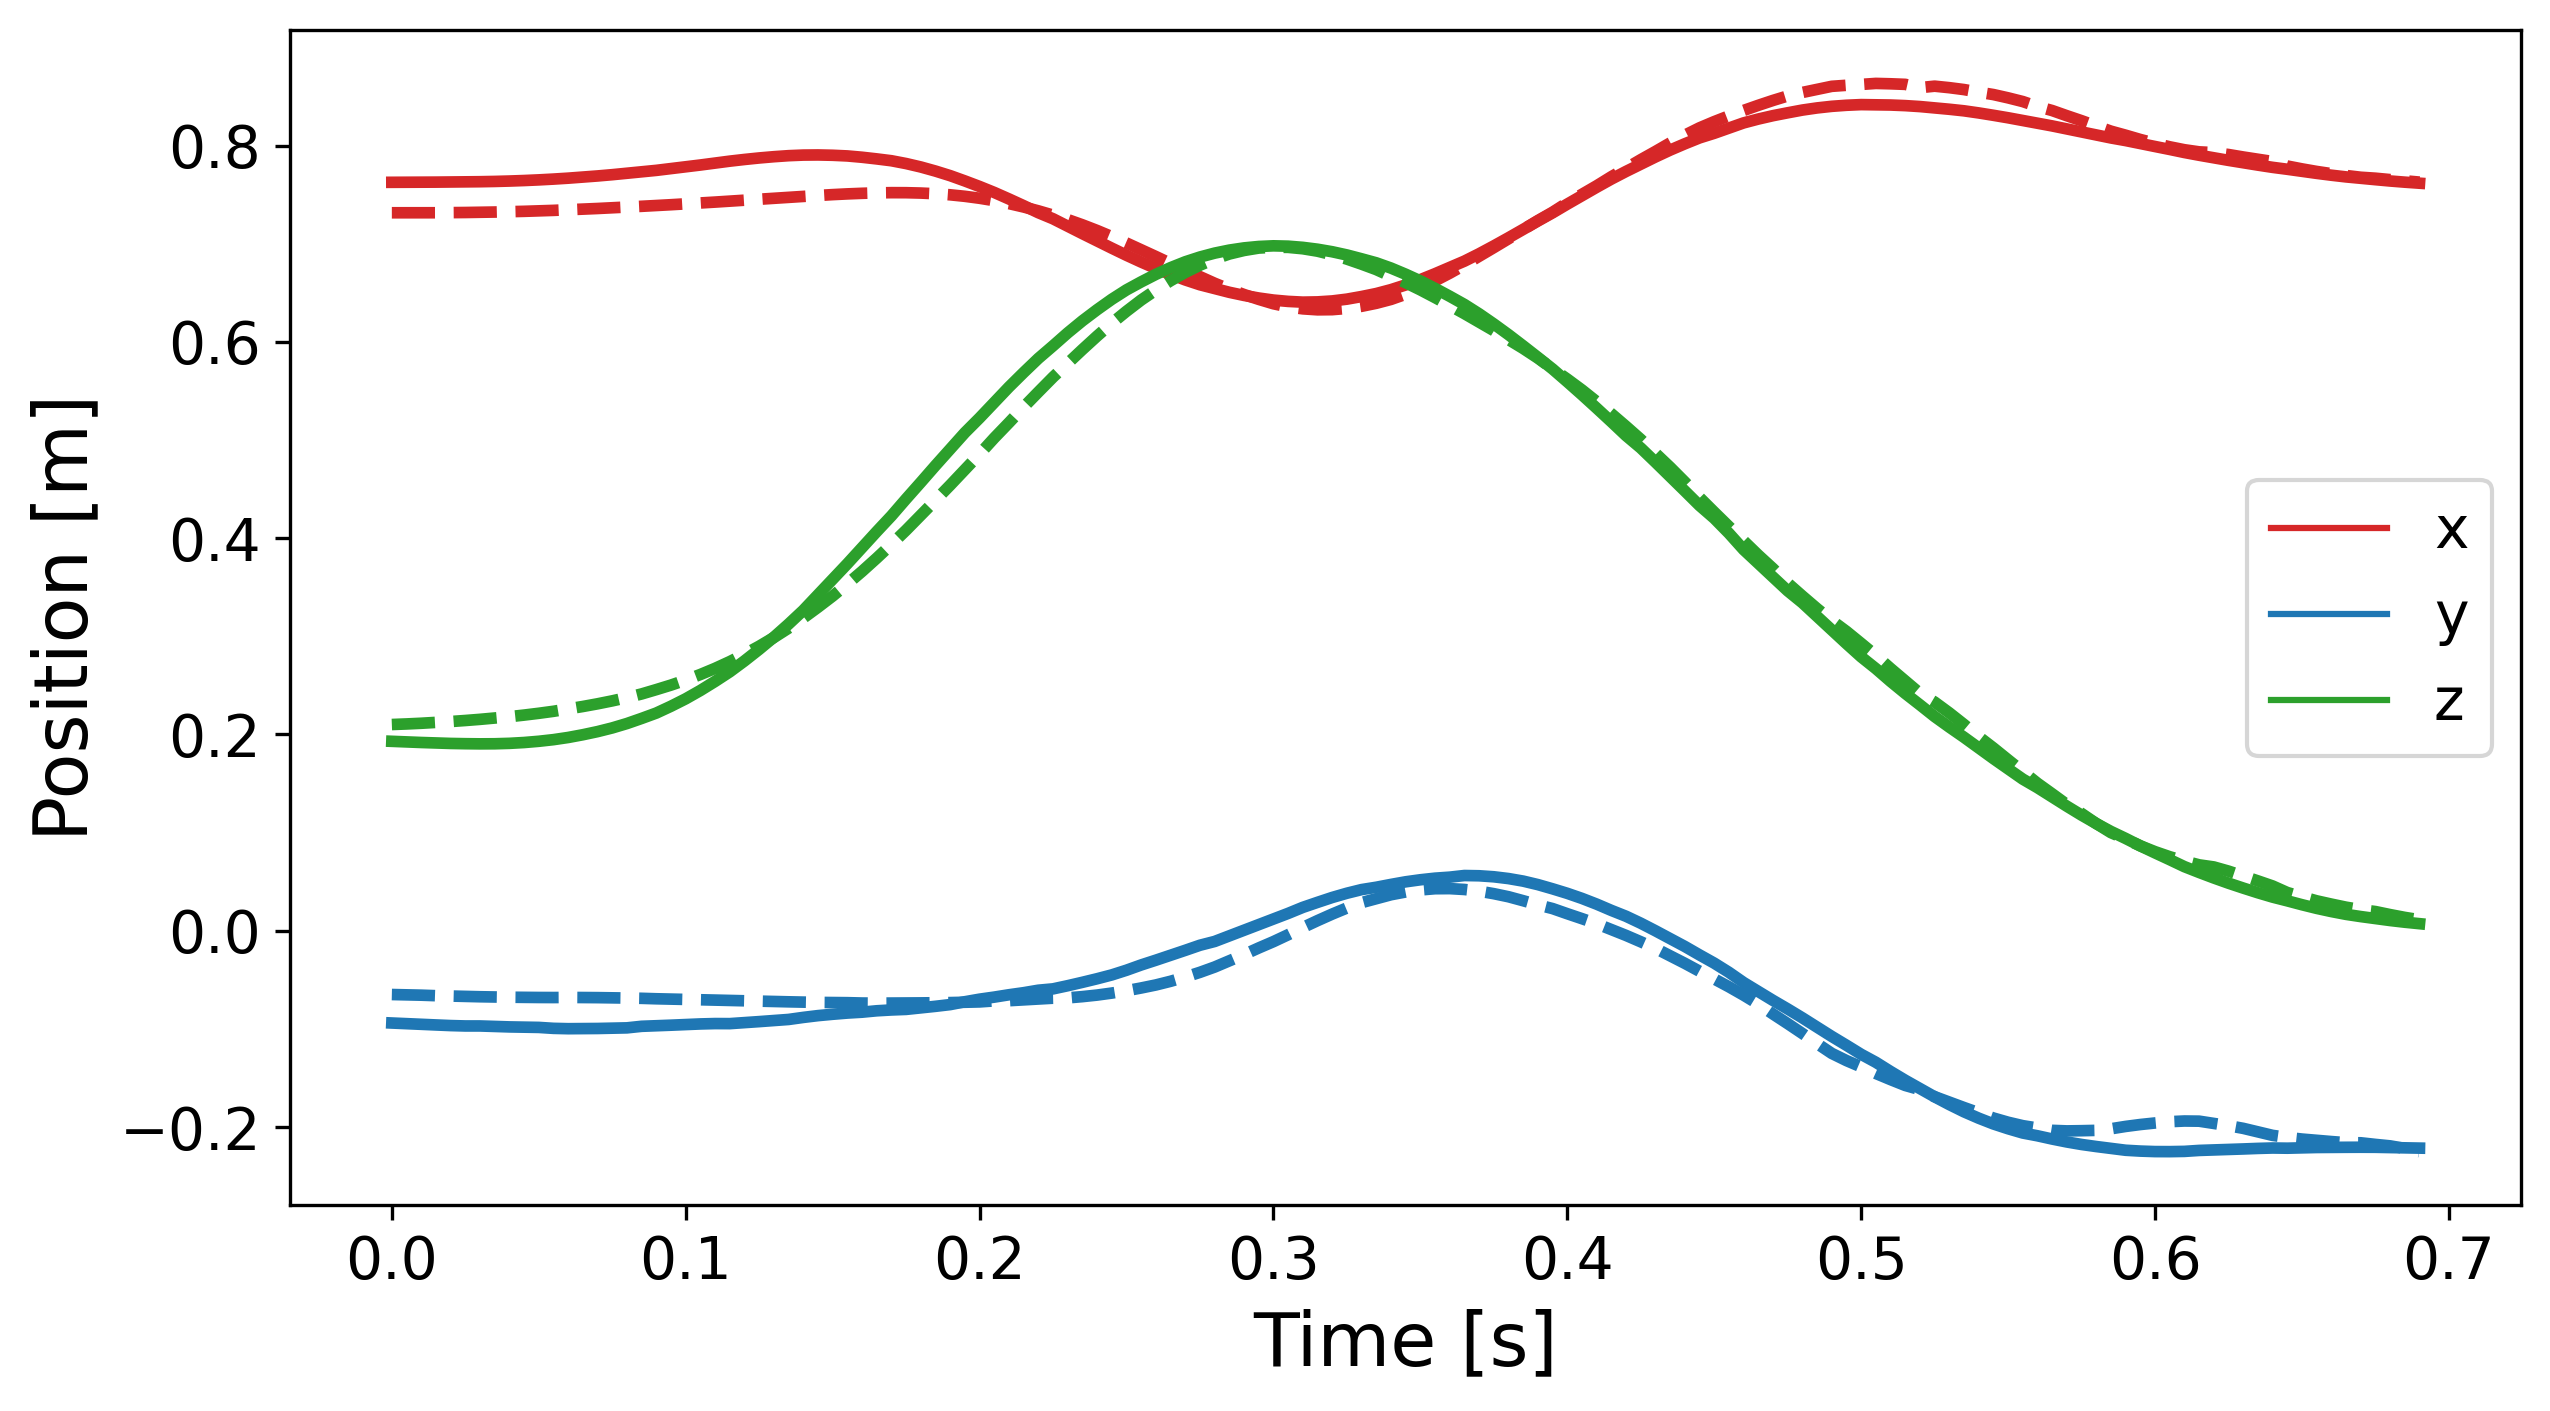
\includegraphics[width=0.85\linewidth]{figs/fttraj.png}
    \vspace{-3mm}
    \caption{\textbf{Initial command fingertip trajectory}: positions of the demonstration fingertip trajectory are dashed, and the robot commanded initial attempt to track the demonstration are solid. The robot fails to track the demonstration motion due to kinematic and dynamic constraints.}
    \label{fig:dmeo_track}
    \vspace{-3mm}
\end{figure}
\begin{figure*}[t]
  \centering
  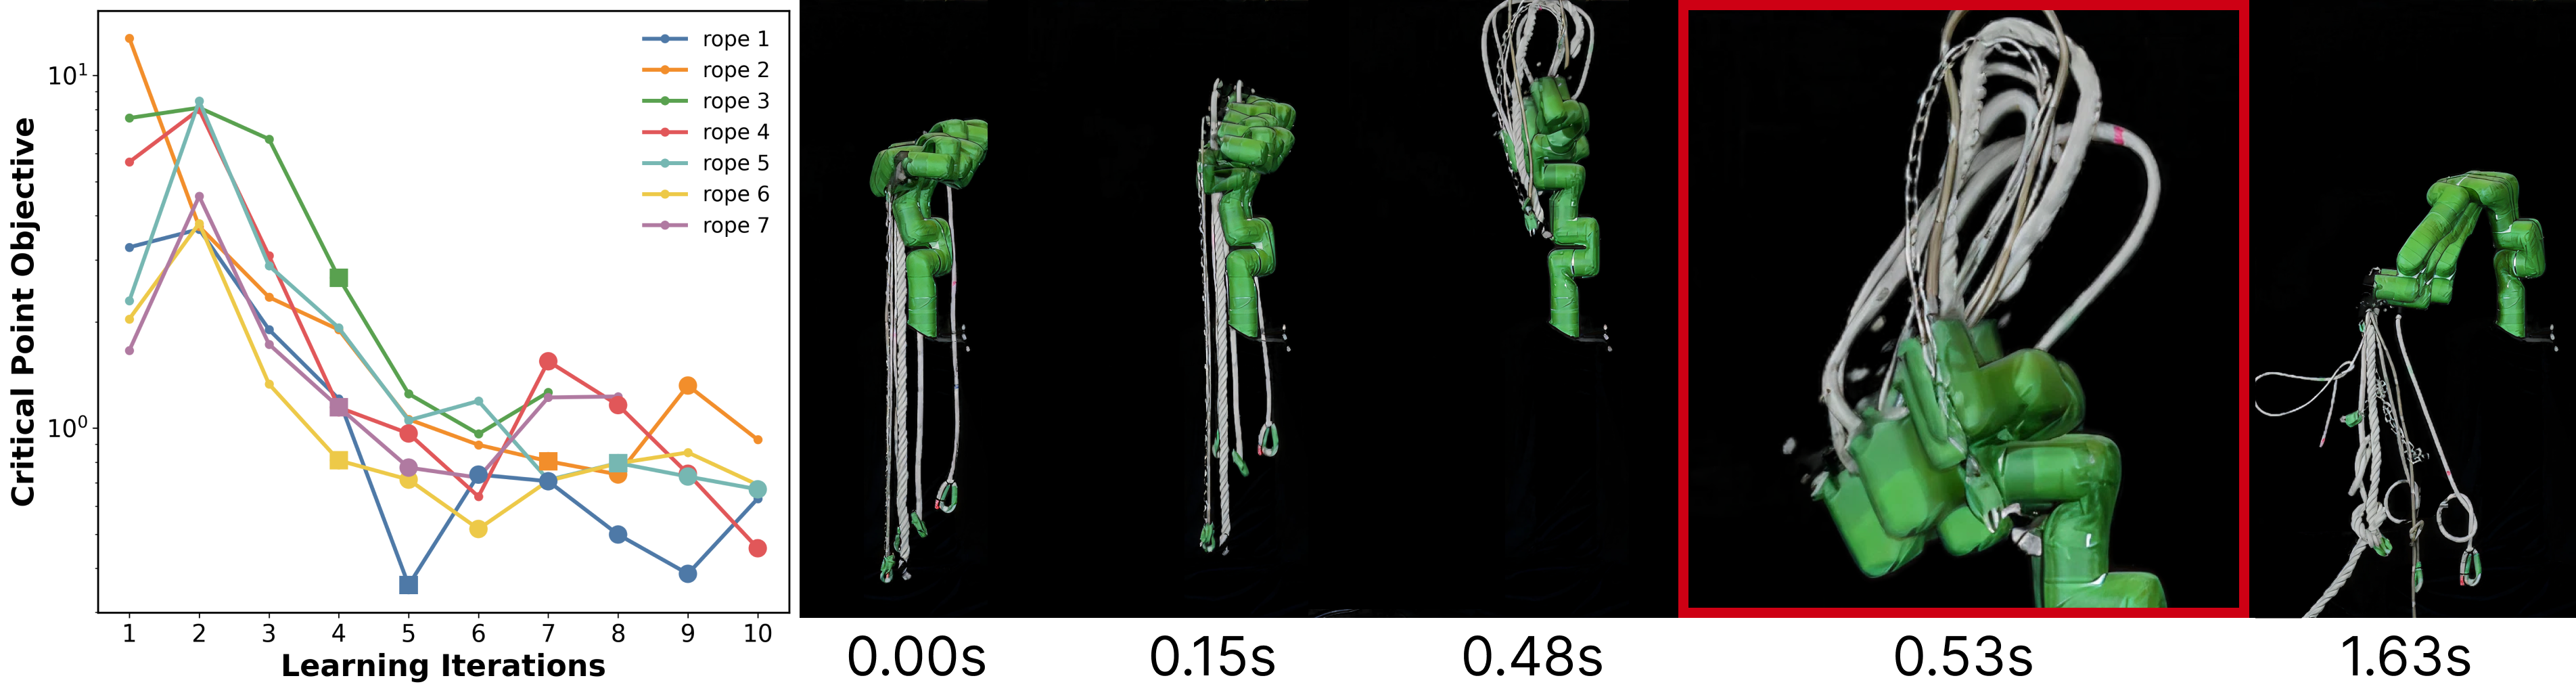
\includegraphics[width=\textwidth]{figs/all_ropes.png}
  \caption{\textbf{Left:} \textit{Critical point} objective for 7 rope types over 10 iterations (rope 3 and 7 end early due to marker tracking failures). Squares represent the first successful flying knot, and every large solid dot represents a subsequent successful knot. \textbf{Right: } Real successful flying knot execution on 7 rope types overlayed. Red highlighted frame is the \textit{critical point}.}
  \label{fig:all_rope_sequence}
  \vspace{-3mm}
\end{figure*}

\subsection{Demonstration Hand Tracking}
For each demonstration type, we apply our initial-guess generation procedure, as described in \cref{sec:initial_guess}, to assess how well the robot performs the task solely by following the demonstrated hand motion. In every rope-demonstration type for rope 1, the robot is unable to tie the flying knot when attempting to follow the demonstration trajectory. However, for certain ropes, such as 4 and 7, following the demonstration nearly achieves a flying knot.

Generating a command to exactly track the demonstrated hand motion is not possible due to the limits of the robot's joint ranges, maximum velocities, accelerations, and torques, as well as the differences between human and robot morphology. An example demonstrated fingertip trajectory and the corresponding initial attempt by the robot are visualized in \cref{fig:dmeo_track}. While the robot can capture the demonstrator's overall motion, it cannot match it exactly, resulting in failures when attempting to tie the flying knot.    


% Furthermore, tracking the demonstration hand motion does not help when executing the task on a different rope since rope dynamics may differ. However, we use tracking of the demonstration hand motion as the initial attempt at the task. 

% Hand motions, which generally follow the demonstration, excite the rope and provide sufficient information for the learning system to know what direction to make command corrections.


\subsection{Weighted Error Objectives}
\label{sec:critical_point_obj}


We compare the performance of the learning algorithm under two objectives: the \textit{critical point} objective (ours) and the equal-weighting objective. The \textit{critical point} objective, which focuses on errors at one point in the trajectory, is described in \cref{sec:critical_point}. The equal-weighting objective weighs rope tracking errors equally along the pre-collision trajectory and is commonly found in trajectory tracking and behavior cloning. 

As seen in \cref{fig:iters}, the critical-point objective aligns the rope state at a single point, at the collision, allowing for different rope motion beforehand, and results in the flying knot success.

% The equal-weighting objective also fails when learning the task with task dynamics different from those in the demonstration. When we use a demonstration given on rope \# 1 and attempt learning across the other 8 ropes, the critical point objective fails to succeed at the task, even when starting with a command that succeeds on rope \# 1. Learning with the critical point objective succeeds at the task on all 9 ropes, both with and without an initially successful command.

Overall, we find that the \textit{critical point} objective is crucial to task success. The equal weighting objective increases errors at the critical point, compared to the critical point objective, to reduce errors at earlier parts of the trajectory that matter less for task success. This error different at the \textit{critical point} for equally-weighted learning causes failure.
% By attending to all aspects of the task, the learning algorithm may become stuck in a local minimum that penalizes errors in task states that are irrelevant. Therefore, the critical-point objective ignores aspects of the demonstration. 

% Specifying this critical-point objective enables learning across variations in rope dynamics, since learning the salient moment yields a closer estimate of the true task objective, which is unknown.



\subsection{Learned Command Success Rate}
Once a successful trajectory is learned, the robot has a 100\% success rate with the resulting learned command. We evaluated this success rate by repeating 40 trials of a learned command and observing no failures. Executions of the successful command are performed immediately after learning, and longer-term changes to the system dynamics, such as rope wear or breaking in (changes to stiffness and damping), and robot motor temperature, might require additional learning iterations.

\subsection{Learning Across Rope Types}
\begin{figure}
    \centering
    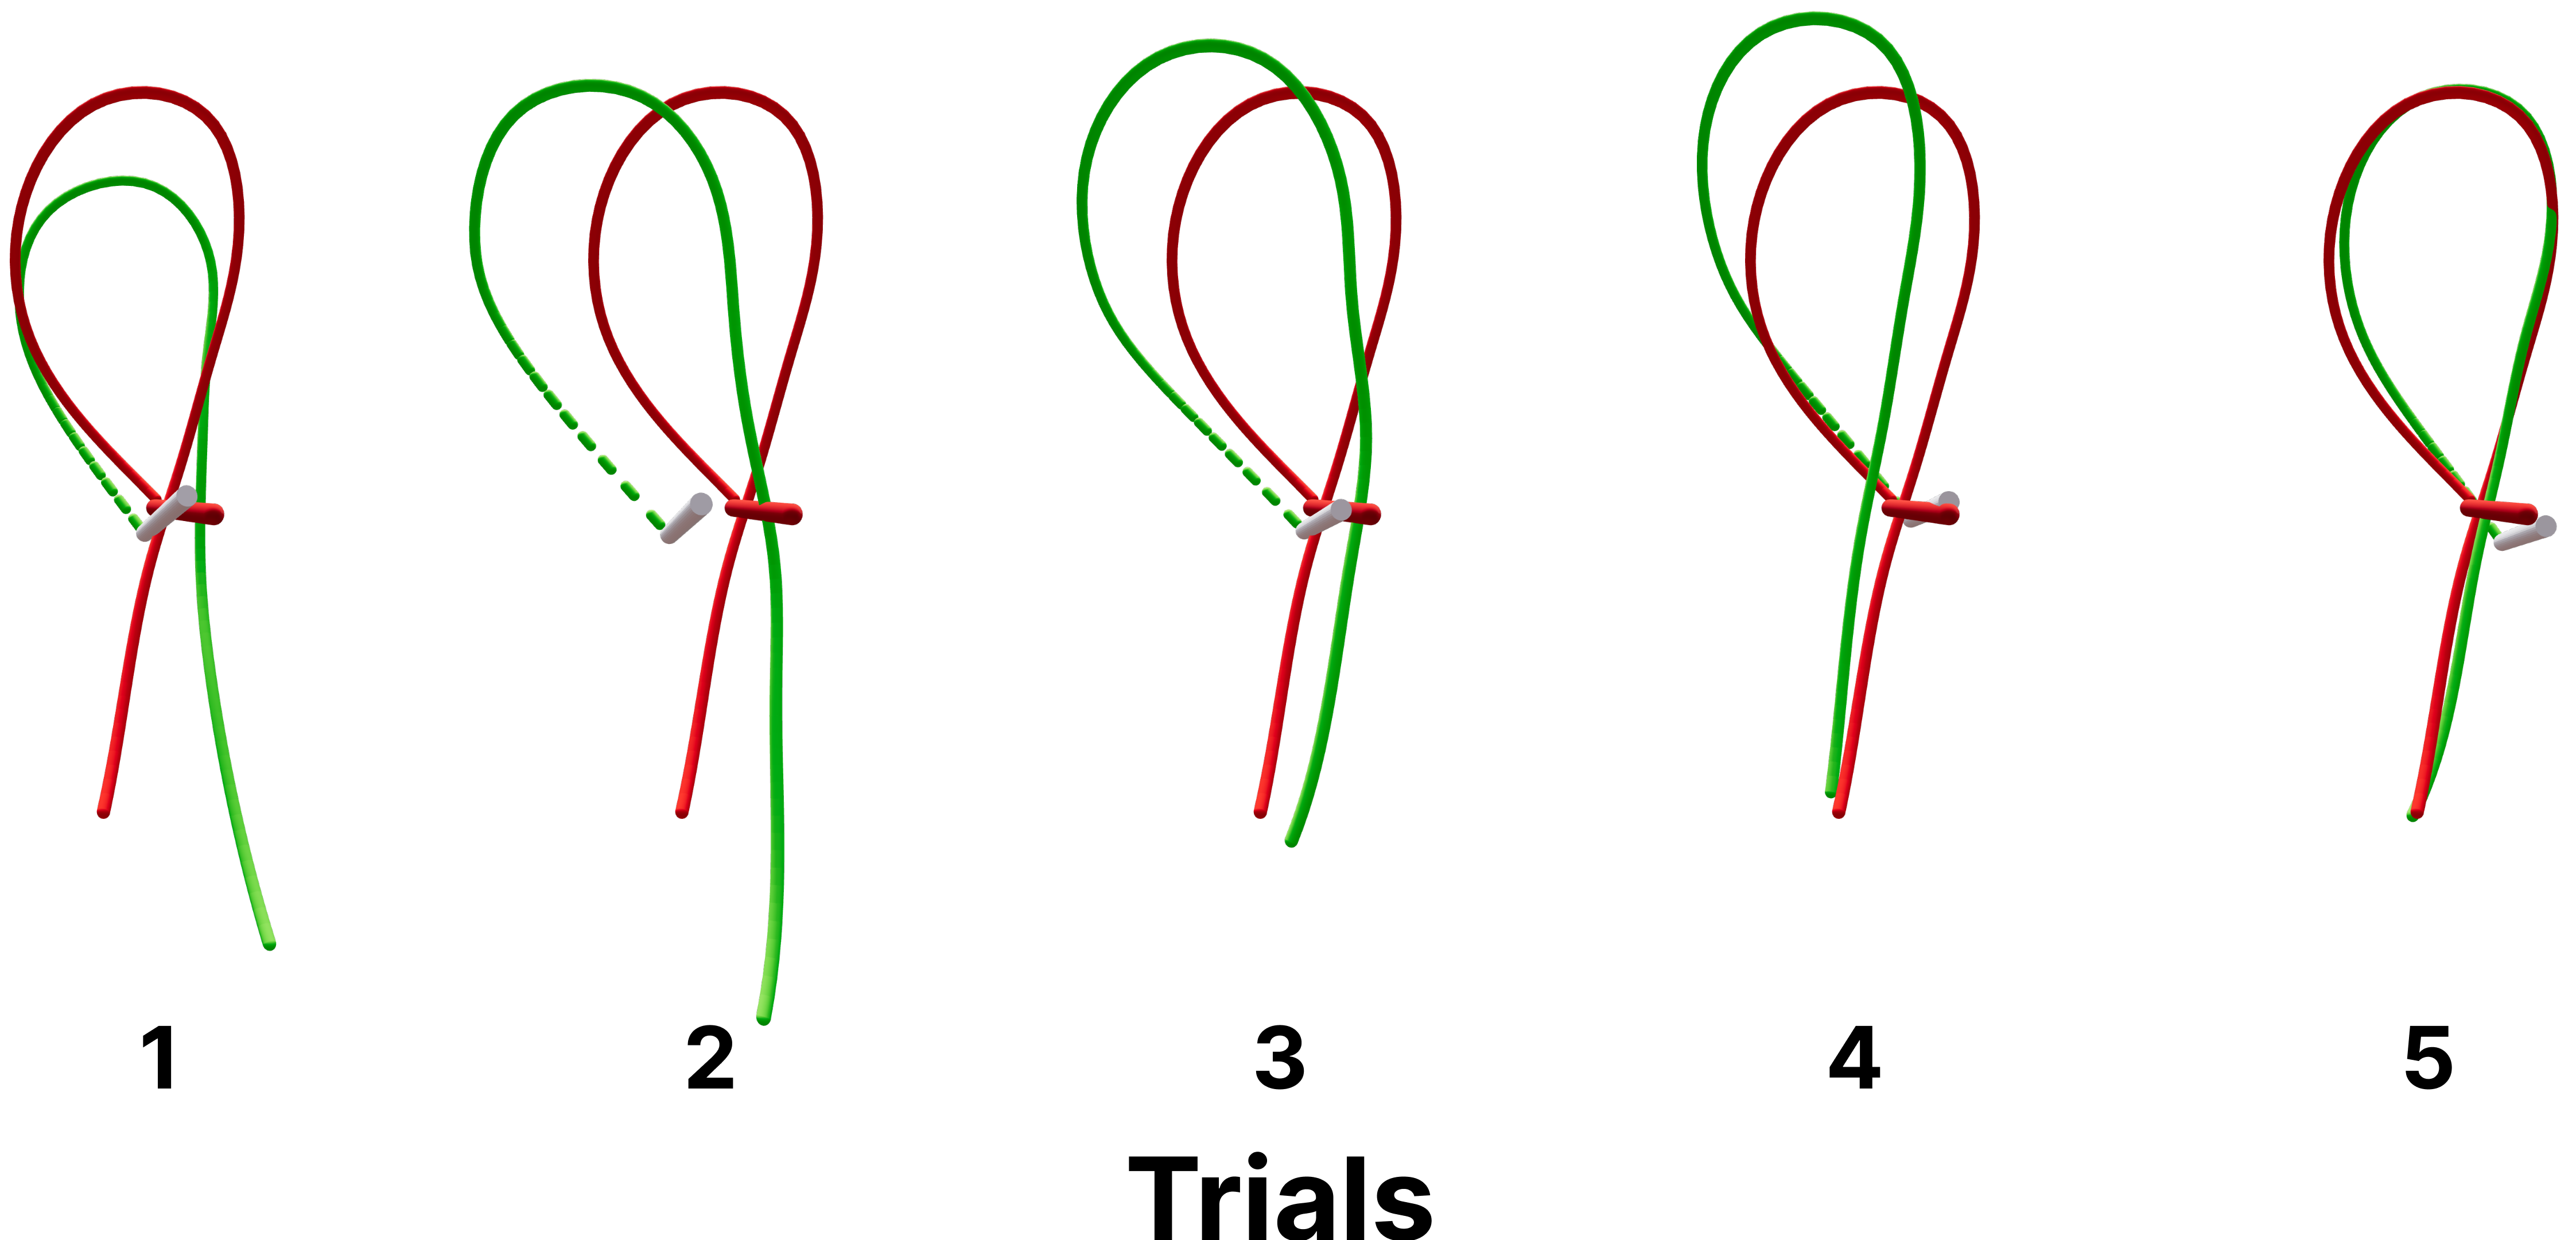
\includegraphics[width=\linewidth]{figs/iterations.png}
    \vspace{-3mm}
    \caption{\textbf{Rope configuration at the \textit{critical point} over learning iterations:} Real rope (green) and goal rope(red) states for 5 iterations of Task-Level ILC where trial 5 resulted in a flying knot.}
    \vspace{-1mm}
    \label{fig:iters}
\end{figure}
We evaluate the learning of the flying knot across 7 different ropes (as shown in \cref{fig:ropes}) to demonstrate the robustness of Task-Level ILC to varying system dynamics. A detailed list of parameters of each rope can be found in Appendix~\cref{sec:rope_params}. In general, ropes span a thickness of 7-25mm, a density of 0.013-0.5 kg/m, and are composed of materials such as cotton, polyester, steel, and latex.
All ropes have a mass fixed to the end with masses selected to allow the human demonstrator to execute the flying knot.

% All ropes have a mass fixed to the end of different sizes corresponding to the stiffness of the rope. Masses were selected to be the minimum required to enable the human demonstrator to make a flying knot. 

% We additionally vary the mass for \ropeone with 0, 10, 20g weights.

Task-Level ILC successfully learns the flying knot on all 7 rope types within 10 trials. The successful flying knot commands are shown in \cref{fig:all_rope_sequence}. Each command starts the rope in a different initial state and performs the upward twisting motion at different speeds. Once the critical moment is reached, all ropes form the same loop shape and allow the knot to be formed. The differences in learned commands show that variation in the rope dynamics requires variation in the command. 
% The learning objective is shown over trials in \cref{fig:all_rope_sequence}. 
As seen in \cref{fig:all_rope_sequence}, the learning algorithm succeeds in fewer trials for some rope types (3, 6, 7) and requires more iterations for others (2, 5), but does not exceed 10 trials on any rope. Overall, the learning process reduces the cost of the \textit{critical point} objective across trials; however, because we are not performing a line search on the real-system objective, the cost can increase after a poor command update, as with rope 4. Furthermore, repeated updates after success can lead to failure, as in trial 9 of rope 2. It is unclear whether additional learning after success leads to convergence to a successful command or to failure, as both outcomes occasionally occur.


% \subsection{Learning Across Rope Types}
% 

% We evaluate learning across 9 rope types with demonstrations on each rope. The measured task error over trials is shown in \cref{fig:learning_curves} with more challenging ropes requiring more trials. 

% We also learn on \ropeone with three sets of mass variations. Changes to the mass at the end of the rope require different commanded motions to succeed, as seen in \cref{fig:mass_diff}.

\subsection{Learning Across Demonstration Variation}
For rope 1, we test whether variations in the demonstration impact learning with the 4 different flying knot demonstration types seen in \cref{fig:demos}. 
% The \textit{critical point} objective is set at the collision point in all types of demonstrations. 
The total demonstration time lengths vary, ranging from 0.69s to 1.04s. The learning algorithm learns the flying knot in all 4 cases.  \cref{fig:4success} shows the learning progression, with Demo Type 2 requiring the most trials. 
% 

\begin{figure}
    \centering
    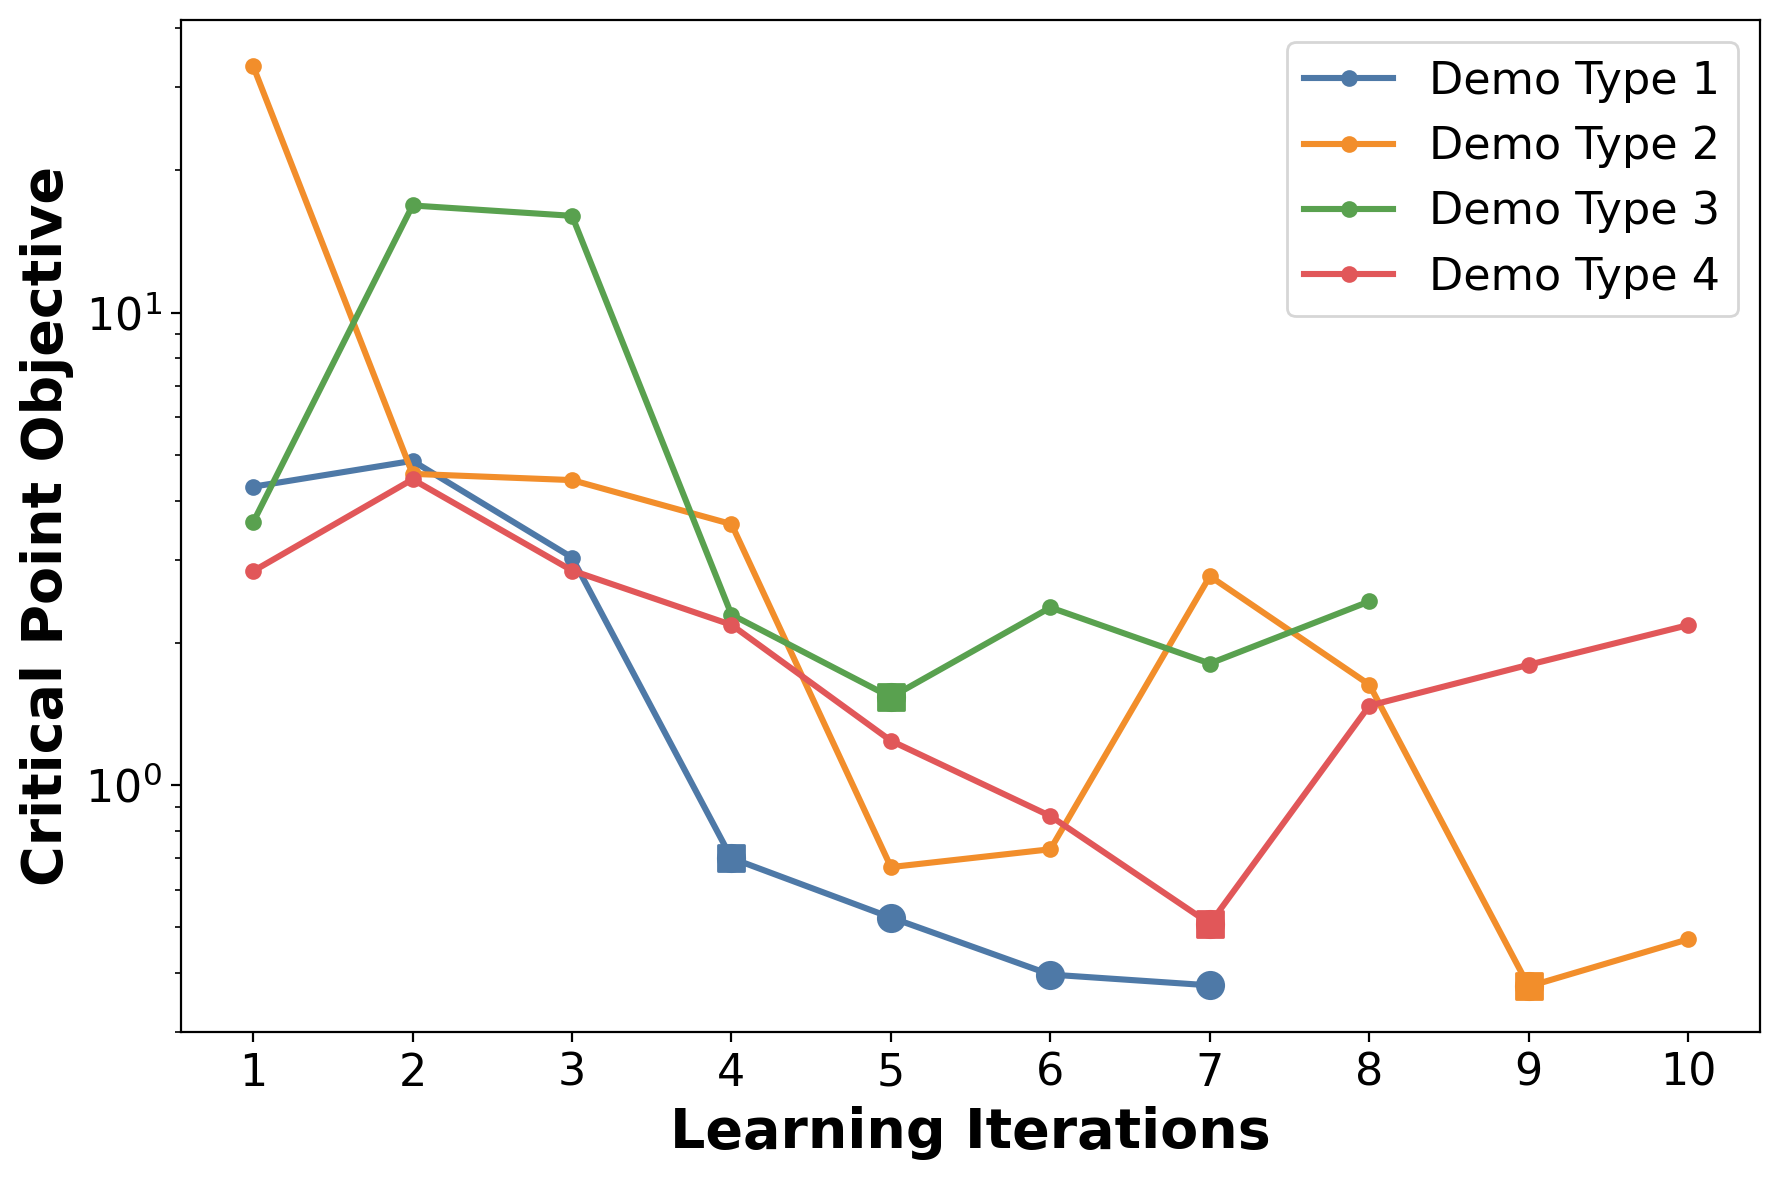
\includegraphics[width=0.75\linewidth]{figs/4demos.png}
    \caption{Learning cost over trials for 4 demonstration types. Large solid dots represent times when the flying knot succeeded, and squares are the first successful command. Learning on Demo Types 1 and 3 is truncated due to rope tracking failures.}
    \label{fig:4success}
    \vspace{-4mm}
\end{figure}

\subsection{Transfer of Learned Command}

Given a demonstration on rope 1 and a successful command on all 7 ropes, we attempt to transfer the learned commands between rope types. The successful command on rope A initiates learning on rope B and has a maximum of 10 trials to improve. A grid of the number of trials required to adapt the command to rope B is shown in \cref{fig:transfer_learning}. For the majority of transfers, the number of trials is larger than 1, showing that the dynamics of the ropes are different enough to require different commands. For rope 7 (9mm latex), no additional learning is required, indicating that rope 7 is more robust to command variations. Additionally, learning fails when commands from ropes 5 and 6 are transferred to ropes 2 and 3. In all three cases, learning iteratively reduces the objective but requires larger adjustments and cannot fully correct the command within the 10 allotted trials. 



\begin{figure}
    \centering
    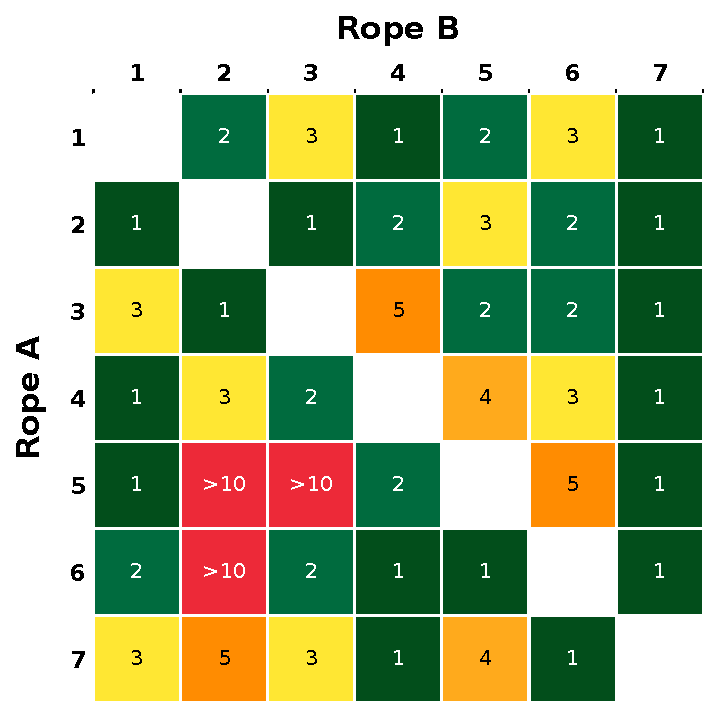
\includegraphics[width=0.75\linewidth]{figs/grid.pdf}
    \vspace{-2mm}
    \caption{Number of trials to transfer a successful command from rope A to rope B. Red cells are for transfer that did not succeed within 10 trials.}
    \label{fig:transfer_learning}
    \vspace{-2mm}
\end{figure}

% Since transferring a single successful command to other ropes fails when using the equal-tracking objective, as shown in \cref{sec:critical_point_obj}, a critical-point objective is a better learning objective for transferring task success across task variations. 
\begin{table}[b]
    \vspace{-3mm}
    \centering
    \caption{Effect of model parameters on learning performance.}
    \label{tab:stiffness_endmass}
    \begin{tabular}{cc|c}
        \toprule
        Stiffness & End Mass & Trials Until Success \\
        \midrule
        $\mathbf{1\times10^{5}}$ & \textbf{5} & \textbf{4} \\
        $1\times10^{5}$ & 0.005  & 6   \\
        $1\times10^{5}$ & 0.05   & 8   \\
        $1\times10^{2}$ & 5      & $>10$ \\
        $1\times10^{3}$ & 5      & 4   \\
        $1\times10^{4}$ & 5      & 4   \\
        \bottomrule
    \end{tabular}
    \vspace{-3mm}
\end{table}


\subsection{Sensitivity to Model Parameters}
\label{sec:model_sensitivity}
ILC can make command corrections in a sample-efficient manner by leveraging a system model. We evaluate the effects of changes to the model parameters by learning on rope 1 with a single demonstration, while varying the system model stiffness $k$ and end mass $m_e$. These parameters were selected for their dominant impact on the model dynamics. In \cref{tab:stiffness_endmass}, we evaluate learning performance with different rope model parameters 
(bold represents the default parameters used across all experiments). 
For order-of-magnitude changes in the model parameters, learning can still succeed. There are cases in which learning fails, such as when stiffness is too low, in which a single command update places the trials in an unrecoverable execution regime. Similarly, for runs with low end-mass values, updates after a successful knot quickly drive the command away from success. 



% We sample parameter values in the following ranges: $k$: [0, 1e7] and $m_e$: [0,100], and test the learning performance on the real system. Can we plot the eigen values of the linearized model to show that it is not very informative when the parameters are in the red region. Make a point about the model gradient information being inaccurate in this range.

% We attempt to identify a best-fit set of parameters by simulating commanded robot motions and comparing them with the real rope motion. The best-fit parameters are optimized via CMA-ES. More details on this parameter identification process can be found in Appendix \ref{sec:parameter_fit}.

% As shown in \cref{fig:model_sensitivity}, learning is robust to large changes in model parameters, suggesting that careful parameter selection is unnecessary for task learning. We apply the parameter fitting procedure to all 12 rope variations and identify the best-fit rope model parameters as seen in \cref{fig:parameter_fit}. However, all results of learning are conducted with a fixed set of ``good enough''  values: .


\section{Discussion}
\subsection{Learning on the Real System}
Task-Level ILC enables task learning on real systems in a sample-efficient manner, using approximate system models to convert real-system errors into command updates. In simulation-based learning methods, such as policy learning on a simulated system model and Sim2Real transfer with domain randomization, issues often arise due to gaps between the system model and the real system. Techniques for model learning attempt to overcome this by adapting the model used for policy optimization with real data, but suffer from limitations of the modeling structure. Domain randomization builds robustness into the policy by optimizing over a range of models. Policy optimization with domain randomization is a worst-case robust control design procedure, where performance is degraded in all situations relative to the performance with an accurate model for that situation.
% Techniques for model learning (and policy optimization on this model) can overcome this by leveraging real-world data, but are limited by the class of model structures for a given system. 

Learning directly on the real system eliminates these issues by allowing the real system to be captured in the learning process. The models used for learning do not need to accurately predict future system states, as illustrated by the large discrepancies between the model predictions and the real rope, yet learning still occurs. These approximate models still provide sufficiently accurate gradient information. As shown in \cref{sec:model_sensitivity}, the learning process is robust to large variations in the parameters, eliminating challenges in accurate model parameter estimation and domain-randomization.


% careful identification of the model parameters is not necessary, 
% Therefore, issues related to model-prediction failures and domain-randomization uncertainty can be addressed by learning on the real system. 


\subsection{Critical Points for Task-Level Learning}
In evaluating the learning system on the flying knot task, we demonstrate that a \textit{critical point} enables learning, robustness, and transfer. In \cref{sec:critical_point_obj}, we show that an equally weighted objective failed to achieve the task because errors at the \textit{critical point} are larger than with a \textit{critical point objective} (as visualized in \cref{fig:critvseq}). 
% The learning algorithm can apply corrections to the entire command to reduce errors at \textit{critical points}. 
% by not optimizing performance on the correct aspects of the task. 
% The critical point serves as a task abstraction that eliminates task-specific dynamics irrelevant to learning and enables the learning algorithm to develop a more general understanding of task errors. 

% Many recent Behavior Cloning (BC) works that learn from human demonstrations of a task can achieve high task performance without critical point knowledge. 
\textit{Would critical point objectives improve Behavior Cloning (BC)?}
BC achieves tasks not by iteratively improving performance but instead by capturing the task distribution with a range of demonstrations. Direct teleoperation of the robot is often required for BC to ensure real system dynamics are captured in demonstrations. In BC, task transfer often struggles across domains and robots. \citet{hu_rac_2025} addresses some of these challenges by leveraging an instructor to guide learning toward subgoals. One can view the highlighted subgoals as
critical points.

% For the flying knot, we manually specify knowledge of the critical points to enable task success, but in general, the critical points of a task may be unknown. The final true task objective of executing a flying knot is ill-posed since a flying knot can exist in many forms, and measures of betterness don't exist. Therefore, we can choose critical points that we deem crucial for task success to approximate the true task objective, giving the learning algorithm a clear objective to achieve.

\subsection{Command Learning}
For tying a flying knot, we are learning a feedforward command. Repeated execution of commands results in reproducible behavior. By learning a feedforward command, the learning problem is reduced to searching for commands as a function of time ($\command(t)$) rather than a general feedback policy ($\command(\state)$). This reduction in the dimensionality of the learning problem comes at a cost of the approach being unable to 
handle unstable systems or situations with large random perturbations.
ILC can be applied to unstable systems that have been stabilized, as in \citet{schoellig_optimization-based_2012}. 




Command learning can also suffer from increased high-frequency corrections, since mechanical systems with energy loss are inherently low-pass filters; inverse models of these systems become high-pass filters. Therefore, learning amplifies high-frequency modeling inaccuracies. Since the robot can only execute smooth, continuous motions, we chose to parametrize the command trajectory using a small number of degrees of freedom. The drawback of this approach is that we cannot correct true high-frequency command errors. 
% command parametrization This reduces the introduction of high-frequency modes into the command signal while also reducing the dimensionality of the learning problem. 

% since high-frequency measurements of task errors often have more noise. This leads to high-frequency noise propagating through the inverse model, distorting the high-frequency components of the command. Since the robot can only execute smooth, continuous motions, we chose to parametrize the command using a low-dimensional representation of 8 Bezier curve knot points. This reduces the introduction of high-frequency modes into the command signal while also reducing the dimensionality of the learning problem. 

Manipulation of deformable objects is well-suited for command learning, as errors are often repeatable, and with energy loss, the system dynamics are usually stable.
% deterministic and the system dynamics are neutrally/fully stable. 

% \subsection{Model Structure}
% \begin{itemize}
%     \item Talk about how we chose model structure, this is open-ended in general
% \end{itemize}

\subsection{Limitations and Future Work}
While our learning system is robust to changes in rope dynamics, different demonstrations, and model parameters, four main failure modes can degrade learning. First, because the system model does not account for collisions, rope collisions with the robot body or the rope handle can cause the inverse model to apply unrecoverable command corrections. Second, the selected \textit{critical point} of the rope collision is sometimes insufficient for fully completing the flying knot, as the rope may tie the knot and execute a follow-through motion, which unties the knot before the rope settles. Similarly, lighter ropes can get caught on the finger surface and be unable to tighten the knot. Third, marker tracking is only accurate up to rope collision, and since we set the \textit{critical point} to be at a fixed time point from the start of motion, if the rope contact happens early, rope state estimation may fail. Lastly, learning can diverge and get stuck in a local minima. Learning divergence occurs more frequently when task errors are too large at the \textit{critical point}, and the model predictions are sufficiently inaccurate.
% \begin{itemize}
%     \item Since the system model does not include collisions, unwanted rope collisions with the robot body or rope handle sometimes cause the inverse model to apply unrecoverable command corrections.
%     \item The selected \textit{critical point} of the rope collision is sometimes insufficient for fully completing the flying knot, as the rope may tie the knot and execute a follow-through motion, which unties the knot before the rope settles. Similarly, lighter ropes can get caught on the finger surface and be unable to tighten the knot.
%     \item Marker tracking is only accurate up to rope collision, and since we set the \textit{critical point} to be at a fixed time point from the start of motion, if the rope contact happens early, rope state estimation may fail. 
%     \item Learning can diverge and get stuck in a local minima. Learning divergence occurs more frequently when task errors are too large at the \textit{critical point}, and the model predictions are sufficiently inaccurate. 
% \end{itemize}

Avenues for future research include autonomous selection of \textit{critical points} from demonstrations or instructional materials, identification of model structures for a given task, and learning from lower-fidelity demonstrations/measurements. Specifying the \textit{critical point} as the rope collision point is a crucial input to our learning approach, and the autonomous identification of these \textit{critical points} will enable a robot to learn efficiently. Potential selection criteria for \textit{critical points} could include: human instruction, changes in contact state; dynamical extrema (position, velocity, acceleration, jerk, curvature, etc.); closest/furthest approach points; dynamic bifurcations/branch points; and dynamical funneling points.   


\section{Conclusion} 
\label{sec:conclusion}
We demonstrate the success of Task-Level Iterative Learning Control for deformable-object manipulation by learning to tie various flying knots in less than 10 trials. We introduce the notion of a critical-point objective and demonstrate task-level learning of unactuated system dynamics. Given a single demonstration of the task, our learning system learns to tie a flying knot across 7 different rope types and 4 demonstration variations. We show that a learned command achieves a 100\% success rate and transfers across most rope types in 2-5 trials. 

% \section*{Acknowledgments}

\bibliographystyle{plainnat}
\bibliography{references}

\clearpage
\appendix

\subsection{Inverse Model Additional Details}
\subsubsection{Inverse Model Parameters}
\label{sec:optimization_params}
\begin{table}[t]
\centering
\caption{Inverse Model Parameters}
\label{tab:invmodelparams}
\begin{tabular}{l c}
\toprule
\textbf{Parameter} & \textbf{Value} \\
\midrule
$w_{\text{control}}$ & $\;0.5\;$ \\
$w_{\text{critical pos}}$ & $\;25\;$ \\
$w_{\text{critical vel}}$ & $\;0.00375\;$ \\
$w_{pc}$ & $\;100\;$ \\
$w_{vc}$ & $\;0.1\;$ \\
$w_{Rc}$ & $\;5\;$ \\
$w_{pft}$ & $\;1\;$ \\
$w_{vft}$ & $\;0.1\;$ \\
$w_{Rft}$ & $\;0.1\;$ \\
$w_{\text{ft velocity}}$ & $\;0.5\;$ \\
$\mathbf{q_{\min}}$ & $[\;-6.28, -1.8, -6.28, -0.19, -6.28, -1.69, -6.28\;]$ \\
$\mathbf{q_{\max}}$ & $[\;6.28, 1.9, 6.28, 3.92, 6.28, 3.14, 6.28\;]$ \\
$\mathbf{\dot q_{\min}}$ & $-[3.14, 3.14, 3.14, 3.14, 3.14, 3.14, 3.14]$ \\
$\mathbf{\dot q_{\max}}$ & $[3.14, 3.14, 3.14, 3.14, 3.14, 3.14, 3.14]$ \\
$\mathbf{\ddot q_{\min}}$ & $-[100, 100, 100, 100, 100, 100, 100]$ \\
$\mathbf{\ddot q_{\max}}$ & $[100, 100, 100, 100, 100, 100, 100]$ \\
$\mathbf{\tau_{\min}}$ & $-[130, 130, 40, 40, 40, 20, 20]$ \\
$\mathbf{\tau_{\max}}$ & $[130, 130, 40, 40, 40, 20, 20]$ \\
\bottomrule
\end{tabular}
\end{table}

We use the shorthand $\|\mathbf{a}\|_{\mathbf{W}}^2 := \mathbf{a}^\top \mathbf{W}\mathbf{a}$. The critical-point objective weights the rope-marker position and velocity errors at $t_c$ with a diagonal matrix
\begin{align*}
    \mathbf{Q} := \operatorname{diag}\!\left(w_{\text{critical pos}}\mathbf{I}_{3N},\; w_{\text{critical vel}}\mathbf{I}_{3N}\right),
\end{align*}
where $N$ is the number of rope markers (links). In general, $w$ is a diagonal cost element for a cost matrix. The control-update regularizer is $\|\commandupdate\|_{\mathbf{R}}^2$ with a diagonal $\mathbf{R}$ applying $w_{\text{control}}$ to the 7 arm-joint update variables. For the follow-through, we penalize the end-effector tracking error in \cref{sec:track_hand} with a time-varying diagonal weight matrix
\begin{align*}
    \mathbf{W}(t) := \operatorname{diag}\!\bigl(w_p(t)\mathbf{I}_3,\; w_R(t)\mathbf{I}_3,\; w_v(t)\mathbf{I}_3\bigr),
\end{align*}

% \begin{align*}
% \mathbf{W}(t) := \begin{bmatrix}
% w_p(t) & 0 & 0 & 0 & 0 & 0 & 0 & 0 & 0 \\
% 0 & w_p(t) & 0 & 0 & 0 & 0 & 0 & 0 & 0 \\
% 0 & 0 & w_p(t) & 0 & 0 & 0 & 0 & 0 & 0 \\
% 0 & 0 & 0 & w_R(t) & 0 & 0 & 0 & 0 & 0 \\
% 0 & 0 & 0 & 0 & w_R(t) & 0 & 0 & 0 & 0 \\
% 0 & 0 & 0 & 0 & 0 & w_R(t) & 0 & 0 & 0 \\
% 0 & 0 & 0 & 0 & 0 & 0 & w_v(t) & 0 & 0 \\
% 0 & 0 & 0 & 0 & 0 & 0 & 0 & w_v(t) & 0 \\
% 0 & 0 & 0 & 0 & 0 & 0 & 0 & 0 & w_v(t)
% \end{bmatrix}.
% \end{align*}




using $(w_p,w_R,w_v)=(w_{pc},w_{Rc},w_{vc})$ at $t=t_c$ and $(w_p,w_R,w_v)=(w_{pft},w_{Rft},w_{vft})$ for $t>t_c$. 

The parameters $\mathbf{q}$ corresponds to the seven robot joint angles with minimum and maximum constratins emposed on the angle, velocity and acceleration. $\tau$ is the predicted joint torque as given by the inverse dynamics of a full robot model. 
All values used in our experiments are listed in \cref{tab:invmodelparams}.

\subsubsection{QP Hand Tracking Objective}
\label{sec:track_hand_qp}
For $t \in [t_c, T]$, we encourage the robot to match the demonstrator's follow-through motion by penalizing the end-effector tracking error. Let $\mathbf{e}_{ft}(t;\commandt)$ denote the end-effector error vector defined in \cref{sec:track_hand}. This error depends nonlinearly on the command through the Bezier spline and forward kinematics. We linearize $\mathbf{e}_{ft}$ about the current command $\command_k(t)$ with respect to a small update $\commandupdate$:
\begin{align}
    \mathbf{e}_{ft}\bigl(t;\command_k(t) + \commandupdate\bigr)
    &\approx
    \mathbf{e}_{ft}\bigl(t;\command_k(t)\bigr) + \mathbf{J}_u(t)\commandupdate, \\
    \mathbf{J}_u(t) &:= \left.\frac{\partial \mathbf{e}_{ft}(t;\commandt)}{\partial \commandt}\right|_{\commandt=\command_k(t)}.
\end{align}
For notational simplicity, we write $\mathbf{e}_{ft}(t) := \mathbf{e}_{ft}(t;\command_k(t))$. We apply a weighted least-squares cost
\begin{align}
    \bigl\|\mathbf{e}_{ft}\bigl(t;\command_k(t) + \commandupdate\bigr)\bigr\|_{\mathbf{W}(t)}^{2}
    &\approx
    \bigl\|\mathbf{e}_{ft}(t) + \mathbf{J}_u(t)\commandupdate\bigr\|_{\mathbf{W}(t)}^{2}.
\end{align}
Expanding and dropping the constant term $\|\mathbf{e}_{ft}(t)\|_{\mathbf{W}(t)}^{2}$ yields a quadratic function of the command update:
\begin{align}
    \|\commandupdate\|_{\mathbf{Q_{ft}}(t),\mathbf{b_{ft}}(t)}^{2}
    &:= \commandupdate^\top \mathbf{Q_{ft}}(t)\commandupdate + \mathbf{b_{ft}}(t)^\top\commandupdate, \\
    \mathbf{Q_{ft}}(t) &= \mathbf{J}_u(t)^\top \mathbf{W}(t)\mathbf{J}_u(t), \\
    \mathbf{b_{ft}}(t) &= 2\,\mathbf{J}_u(t)^\top \mathbf{W}(t)\mathbf{e}_{ft}(t).
\end{align}


% \begin{verbatim}
% # (p_t - p_d).T Q (p_t - p_d)
% # p_t approx = p + J(dp)
% # (Jp - p_d).T Q (Jp - p_d)
% # (Jp - p_d).T (QJp - Qp_d)
% # p'J'QJp - p_d'QJp - p'J'Qp_d + p_d'Qp_d
% # p'J'QJp - 2p_d'QJp + p_d'Qp_d
% # A = J'QJ  b = -2p_d'QJ c = p_d'Qp_d
% # p'Ap + bp + c
% \end{verbatim}
\begin{table*}[t]
    \centering
    \caption{List of Rope parameters}
    \label{tab:rope_id}
    \small
    \setlength{\tabcolsep}{6pt}
    \begin{tabular}{c l c c c c}
        \toprule
        \textbf{ID} &
        \textbf{Name} &
        \textbf{Material} &
        \textbf{Diameter [mm]} &
        \textbf{Density [kg/m]} &
        \textbf{End Weight [g]} \\
        \midrule
        1 & \#10 Sash Spot Cord   & Cotton & 9  & 0.040 & 18 \\
        2 & \#14 Spot Cord        & Cotton & 12 & 0.081 & 80 \\
        3 & Soft Braided          & Cotton & 15 & 0.076 & 80 \\
        4 & Shoe Lace             & Cotton & 7  & 0.014 & 5  \\
        5 & Thick Twisted         & Cotton & 25 & 0.139 & 50 \\
        6 & 3/8" Chain            & Steel  & 20 & 0.514 & 50 \\
        7 & 3/8" Surgical Tubing  & Latex  & 9  & 0.026 & 18 \\
        \bottomrule
    \end{tabular}
    \label{table:params}
\end{table*}
\subsection{Rope Parameters}
\label{sec:rope_params}
Rope types were selected to evaluate the algorithm robustness to diameter, material, and density. Weights were chosen to enable human demonstrator to perform the demonstration successfully. A full list of parameters for each rope type used in evaluation can be found in \cref{table:params}. 

\subsection{Rope Dynamics Model}
\label{sec:dynamics_model}
We model the rope as a serial chain of $N$ point masses in maximal coordinates and simulate it with the first-order variational integrator described by \citet{lavalle_linear-time_2021}. In maximal coordinate dynamics formulations, each link of the rigid body mechanism is tracked in a global frame. Interactions between links such as joints or contacts are represented explicitly in an optimization problem solved at each timestep. Similarly, in our rope model, we do not track the joint angles between links but instead only track the global position and velocity of each link, then impose constraints to enforce the serial structure of the rope. Let $\mathbf{p}_k^{(i)}\in\mathbb{R}^3$ and $\mathbf{v}_k^{(i)}\in\mathbb{R}^3$ denote the position and velocity of link $i\in\{1,\dots,N\}$ at discrete timestep $k$. We stack all link positions and velocities as
\begin{align*}
    \mathbf{p}_k &:= \begin{bmatrix} {\mathbf{p}_k^{(1)}}^\top & \cdots & {\mathbf{p}_k^{(N)}}^\top \end{bmatrix}^\top \in \mathbb{R}^{3N}, \\
    \mathbf{v}_k &:= \begin{bmatrix} {\mathbf{v}_k^{(1)}}^\top & \cdots & {\mathbf{v}_k^{(N)}}^\top \end{bmatrix}^\top \in \mathbb{R}^{3N},
\end{align*}
and define the rope state (used throughout the paper) as $\state_k := \begin{bmatrix}\mathbf{p}_k^\top & \mathbf{v}_k^\top\end{bmatrix}^\top$. The integrator also introduces constraint multipliers $\boldsymbol{\lambda}_k$, and we denote the full maximal-coordinate variable by $\mathbf{z}_k := \begin{bmatrix}\mathbf{p}_k^\top & \mathbf{v}_k^\top & \boldsymbol{\lambda}_k^\top\end{bmatrix}^\top$. In \cref{eq:dynamics}, $\mathbf{z}_0$ denotes the initial rope configuration, with $\boldsymbol{\lambda}_0=\mathbf{0}$.

The rope is driven by the robot fingertip position $\mathbf{p}_{\mathrm{tip},k}\in\mathbb{R}^3$, which we treat as an input. We enforce inextensibility via fixed-distance constraints between adjacent links of the rope and between the fingertip and the first link:
\begin{align*}
    g(\mathbf{p}_k, \mathbf{p}_{\mathrm{tip},k})
    &:=
    \begin{bmatrix}
        \|\mathbf{p}_k^{(1)} - \mathbf{p}_{\mathrm{tip},k}\|^2 - l^2 \\
        \|\mathbf{p}_k^{(2)} - \mathbf{p}_k^{(1)}\|^2 - l^2 \\
        \vdots \\
        \|\mathbf{p}_k^{(N)} - \mathbf{p}_k^{(N-1)}\|^2 - l^2
    \end{bmatrix}
    = \mathbf{0}.
\end{align*}
Let $\mathbf{G}(\mathbf{p}_k, \mathbf{p}_{\mathrm{tip},k}) := \frac{\partial g}{\partial \mathbf{p}}(\mathbf{p}_k, \mathbf{p}_{\mathrm{tip},k}) \in \mathbb{R}^{N\times 3N}$ be the constraint Jacobian, and let $\boldsymbol{\lambda}_k\in\mathbb{R}^{N}$ be the corresponding Lagrange multipliers, so that constraint forces on the links are $\mathbf{G}^\top \boldsymbol{\lambda}_k$.

The mass matrix is block diagonal,
\begin{align*}
    \mathbf{M}_{\mathrm{mass}} := \operatorname{diag}\!\left(m\mathbf{I}_{3(N-1)},\; m_e \mathbf{I}_3\right)\in\mathbb{R}^{3N\times 3N},
\end{align*}
and we collect gravity and internal bending forces (stiffness $k$ and damping $b$) into a single force vector $\mathbf{f}(\mathbf{p},\mathbf{v})\in\mathbb{R}^{3N}$. With these definitions, a single timestep of the variational integrator can be written as an implicit system in the unknowns $(\mathbf{p}_{k+1},\mathbf{v}_{k+1},\boldsymbol{\lambda}_{k+1})$:
\begin{align}
    \mathbf{0} &=
    \mathbf{p}_{k+1} - \mathbf{p}_k - \Delta t\, \mathbf{v}_{k+1},
    \label{eq:rope_vi_pos}\\
    \mathbf{0} &=
    \mathbf{M}_{\mathrm{mass}}(\mathbf{v}_{k+1}-\mathbf{v}_k)
    - \Delta t\,\mathbf{f}(\mathbf{p}_{k+1}, \mathbf{v}_{k+1})
    \nonumber\\
    &\quad
    - \Delta t\,\mathbf{G}(\mathbf{p}_{k+1}, \mathbf{p}_{\mathrm{tip},k+1})^\top \boldsymbol{\lambda}_{k+1},
    \label{eq:rope_vi_dyn}\\
    \mathbf{0} &= g(\mathbf{p}_{k+1}, \mathbf{p}_{\mathrm{tip},k+1}).
    \label{eq:rope_vi_con}
\end{align}
We solve \cref{eq:rope_vi_pos,eq:rope_vi_dyn,eq:rope_vi_con} with Newton's method at each timestep to roll out the rope trajectory, which defines the simulator $f$ used in \cref{eq:dynamics}.

To compute the local linear model used in the inverse-model QP, we differentiate an implicit system. Let $\tilde{\mathbf{z}}$ stack all per-timestep unknowns $(\mathbf{p}_k,\mathbf{v}_k,\boldsymbol{\lambda}_k)$ over the horizon and let $\tilde{\mathbf{u}}$ stack the driven fingertip positions $\mathbf{p}_{\mathrm{tip},k}$. Concatenating \cref{eq:rope_vi_pos,eq:rope_vi_dyn,eq:rope_vi_con} over time yields an implicit residual $\tilde f(\tilde{\mathbf{z}},\tilde{\mathbf{u}})=\mathbf{0}$. For a solution $(\tilde{\mathbf{z}}^\ast,\tilde{\mathbf{u}}^\ast)$, the implicit function theorem gives
\begin{align}
    \frac{\partial \tilde{\mathbf{z}}^\ast}{\partial \tilde{\mathbf{u}}}
    =
    -\left(\frac{\partial \tilde f}{\partial \tilde{\mathbf{z}}}\right)^{-1}
    \frac{\partial \tilde f}{\partial \tilde{\mathbf{u}}}.
    \label{eq:rope_ift}
\end{align}
In practice we do not form the inverse explicitly and instead solve linear systems with the KKT Jacobian $\frac{\partial \tilde f}{\partial \tilde{\mathbf{z}}}$. We implement the residual and its derivatives in Drake using automatic differentiation \cite{drake}, and apply the chain rule through the Bezier spline and forward kinematics to obtain the system-model linearization $\mathbf{M}$ in \cref{eq:dyn}.
% Starting with the principle of least action where $\mathcal{L} = \mathcal{T}-\mathcal{V}$ is the Lagrangian of our dynamics, we can find the unforced dynamics of the system by minimizing the following integral:
% \begin{align}
%    S_{\text{unforced}} = \int_{t_1}^{t_N}\mathcal{L} (\mathbf{x}(t),  \mathbf{\dot x} (t)) dt
% \end{align}

% where $\mathcal{T}$ is the kinetic energy, $\mathcal{V}$ is the potential energy, and $\mathbf{x}$ is the continuous trajectory of the system. 

% Since our system only has translational bodies we can define the following quantities where the superscript corresponds each link in the rope:
% \begin{align*}
%    \mathbf{x} &= \begin{bmatrix}
%       x^{(1)}\\
%       y^{(1)}\\
%       z^{(1)}\\
%       x^{(2)}\\
%       y^{(2)}\\
%       z^{(2)}\\
%       \vdots\\
%       x^{(N)}\\
%       y^{(N)}\\
%       z^{(N)}\\
%    \end{bmatrix}
%    \mathbf{v} = \begin{bmatrix}
%       \dot x^{(1)}\\
%       \dot y^{(1)}\\
%       \dot z^{(1)}\\
%       \dot x^{(2)}\\
%       \dot y^{(2)}\\
%       \dot z^{(2)}\\
%       \vdots\\
%       \dot x^{(N)}\\
%       \dot y^{(N)}\\
%       \dot z^{(N)}\\
%    \end{bmatrix}
%    \mathbf{\lambda} = \begin{bmatrix}
%       \lambda^{(1)}\\
%       \lambda^{(2)}\\
%       \vdots\\
%       \lambda^{(N-1)}\\
%    \end{bmatrix}\\
%    \mathbf{M} &= \begin{bmatrix}
%       m\\
%       &m\\
%       && \ddots\\
%       &&&m\\
%       &&&&m_{end}\\
%       &&&&&m_{end}\\
%       &&&&&&m_{end}\\
%    \end{bmatrix}
%    \mathbf{z} = \begin{bmatrix}
%       \mathbf{x}\\\mathbf{v}\\\mathbf{\lambda}
%    \end{bmatrix}\\
%    \mathbf{e_z} &= \begin{bmatrix}
%       0 & 0 & g & &0 &0&\hdots & g
%    \end{bmatrix}
% \end{align*}

% Where $\mathbf{x}$ is position, $\mathbf{v}$ is velocity, $\mathbf{\lambda}$ is the constraint force, $\mathbf{M}$ is the mass matrix, and $\mathbf{z}$ is our system state vector. $\mathbf{e_z}$ is a helper vector to project onto the gravity vector. Now we can define $\mathcal{T}$ and $\mathcal{V}$ for our system:
% \begin{align*}
%    \mathcal{T} &= \frac{1}{2} \mathbf{v^T M v}\\
%    \mathcal{V} &= \mathbf{e_z}^T \mathbf{M x}\\
% \end{align*}

% The dynamics of the full rope system can be found by minimizing the following integral:
% \begin{align}
%    S(\mathbf{z}) = \int_{t_1}^{t_N} \left(\frac{1}{2} \mathbf{v}^T M \mathbf{v} - \mathbf{e_z}^T M \mathbf{x} \right)dt + \int_{t_1}^{t_N} \mathbf{\lambda}^T \mathbf{g(\mathbf{x})} dt
% \end{align}
% Here $\mathbf{g(\mathbf{x})}$ is the distance constraints enforced between sequential particles where $\mathbf{g(\mathbf{x})}=0$ must be satisfied.
% \begin{align}
%    r^{(i)} = \begin{bmatrix}
%       x^{(i)} & y^{(i)} & z^{(i)}
%    \end{bmatrix}^T\\
%    \mathbf{g(x)} = \begin{bmatrix}
%       {r^{(1)}}^T r^{(2)} - l^2\\
%       {r^{(2)}}^T r^{(3)} - l^2\\
%       \vdots\\
%       {r^{(N-1)}}^T r^{(N)} - l^2\\
%    \end{bmatrix}
% \end{align}

% The control input for the rope is a kinematic trajectory of the hand imposing an additional distance constraint $g$ between the first particle and the finger tip. The position of the hand at each time step can either be parameterized in world coordinates directly or mapped through the robot joint forward kinematics. 

% Since we are using a variational integrator, we directly discretize the least-action integral into a sum with a backwards euler integrator:

% \begin{align}
%    \mathbf{v_k} &= \frac{\mathbf{x_{k+1}}-{\mathbf{x_k}}}{\Delta t}\\
%    S_d(\mathbf{z_k}) &= \sum_{k=1}^{N-1} \left(\frac{1}{2} \mathbf{v_k^T} \mathbf{M}\mathbf{v_k} - \mathbf{e_z}^T M \mathbf{x_k} + \mathbf{\lambda_k}^T \mathbf{g(x_k)} \right) \Delta t
% \end{align}
% We then know that our dynamics are satisfied when $\nabla_{\mathbf{z_k}} S_d(\mathbf{z_k}) = 0$. 


\subsection{Command Parametrization}
\label{sec:bezier}
The Bezier trajectory $\mathcal{B}$ is parametrized by the 8 knot points $\commandt \in \mathbb{R}^{10\times 8}$ equally spaced in the time interval from 0 to $T$. $\mathcal{B}$ is defined as follows, with $b_i$ representing the Bernstein basis functions:
\begin{align*}
\mathcal{B}(\commandt, T)
&= \sum_{i=0}^{N} \command_i \, b_i^{N}\!\left(\frac{t}{T}\right), \quad t \in [0, T] \\
b_i^{N}(s)
&= \binom{N}{i} s^{i} (1 - s)^{N-i}, \quad s \in [0,1].
\end{align*}

\subsection{Demonstration Timing Selection}
\label{sec:demoselect}
Given a full demonstration of the flying knot, we select a time window from $t_0$ to $t_f$ to limit demonstration motion to between the start of hand motion and the end of the follow-through motion. We select these times given a manually annotated rope collision time $t_c$ with the following search procedure:
\begin{enumerate}
    \item Select a temporary range $\tilde t_0$ and $\tilde t_f$ that excludes noisy data from the human picking up and placing the rope on the floor.
    \item Search for maximum hand velocity in the range $[\tilde t_0, \tilde t_f]$ and label as $t_{\text{peak}}$
    \item Step backwards in time from $t_{\text{peak}}$ and update $\tilde t_0$ to the first point when the hand velocity is near-zero (3\% of velocity at $t_{\text{peak}}$).
    \item Set $t_f=t_c + 35\text{ms}$  as a fixed follow through time length.
    \item Integrate along the hand path motion between $\tilde t_0$ and $t_f$, then set $t_0$ to the time when 5\% of the total path length is traveled.
\end{enumerate}
$h(t)$ is then defined as 3D pose trajectory of the hand between $t_0$ and $t_f$. $\state^{\text{demo}}(t)$ is the rope trajectory from $t_0$ to $t_c$. Each demonstration type has a different execution speed and overall time length. 

\begin{table}[b]
\centering
\caption{Demonstration Tracking Parameters}
\label{tab:ikparams}
\begin{tabular}{l c}
\toprule
\textbf{Parameter} & \textbf{Value} \\
\midrule
$\mathbf{q_{\min}}$ & $[\;-6.28, -1.8, -6.28, -0.19, -6.28, -1.69, -6.28\;]$ \\
$\mathbf{q_{\max}}$ & $[\;6.28, 1.9, 6.28, 3.92, 6.28, 3.14, 6.28\;]$ \\
$\mathbf{\dot q_{\min}}$ & $-[3.14, 3.14, 3.14, 3.14, 3.14, 3.14, 3.14]$ \\
$\mathbf{\dot q_{\max}}$ & $[3.14, 3.14, 3.14, 3.14, 3.14, 3.14, 3.14]$ \\
$\mathbf{\ddot q_{\min}}$ & $-[100, 100, 100, 100, 100, 100, 100]$ \\
$\mathbf{\ddot q_{\max}}$ & $[100, 100, 100, 100, 100, 100, 100]$ \\
$w_j$ & $5.0 \times 10^{-7}$ \\
$w_p$ & $\;10\;$ \\
$w_R$ & $\;0.2\;$ \\
$w_v$ & $\;0.5\;$ \\
$z_{\min}$ & $\;1.2\;$ \\
\bottomrule
\end{tabular}
\end{table}
\subsection{Demonstration Tracking}
\label{sec:track_hand}
The first 7 rows of $\mathbf{q}(t)$ correspond to the robot joint trajectory and the remaining 3 rows correspond to the robot base location. $\mathbf{e}_h(t)$ is the end-effector tracking error with respect to the desired fingertip trajectory $h(t)$ weighted by the cost matrix $\mathbf{W}_h$:
\begin{align*}
\mathbf{e}_h(t) :=
\begin{bmatrix}
\mathbf{p}_{\mathrm{tip}}(t)-\mathbf{p}_h(t)\\
\operatorname{Log}\!\bigl(\mathbf{R}_h(t)^\top \mathbf{R}_{\mathrm{tip}}(t)\bigr)\\
\dot{\mathbf{p}}_{\mathrm{tip}}(t)-\dot{\mathbf{p}}_h(t)
\end{bmatrix}\\
\mathbf{W}_h := \operatorname{diag}(w_p\mathbf{I}_3,\;w_R\mathbf{I}_3,\;w_v\mathbf{I}_3),
\end{align*}
with $\mathbf{p}_{\mathrm{tip}}(t)$, $\mathbf{R}_{\mathrm{tip}}(t)$, and $\dot{\mathbf{p}}_{\mathrm{tip}}(t)$ given by the robot forward kinematics $\mathcal{K}$. Values for $w_p, w_R, w_v$ can be found in \cref{tab:ikparams}. While the joint dynamics limits between \cref{tab:ikparams} and \cref{tab:invmodelparams} are the same. The overall objective in the demonstration tracking is equally tracking the hand motion without any critical point weighting, therefore, the cost terms are applied equally throughout the hand motion.

The $z_{\mathrm{tip}}$ constraint specifies that the initial configuration of the robot at $t_0$ must have enough distance for the rope to dangle without hitting the floor. 












% Recent work in imitation learning such as from \cite{hannus2024dynamic, hu_rac_2025,nair2017combining} have demonstrated success in manipulation of rope and cloth, however, much of these frameworks are limited to quasi-static tasks. To address dynamic tasks, \citet{chi_iterative_2022} and \citet{zhang_robots_2024} show systems for learning to manipulate planar and constrained ropes in dynamic settings. However, both of these systems rely on strong learned priors from large simulated data collection. 

% To learn the highly-dynamic \textit{Flying Overhand Knot}, we first attempted to copy the hand motion given by the demonstrator. This did not succeed due to the difference in kinematics and dynamics between the demonstrator and the robot. Next, we attempted to learn the flying knot in simulation and transfer our policy to the real robot. This did not succeed due to significant modeling errors in both the robot and rope models especially during fast motions. Therefore, we needed a way to learn this task directly on the real robot to minimize both the Human2Robot and Sim2Real gaps. 

% However, many current learning approaches rely in large parameter models, policies and task representations, requiring large amounts of data to train. This makes learning on the real robot often intractable. 

% The key to learning on the real robot is to dramatically reduce the dimensionality of the learning problem. We make learning tractable by leveraging a number of dimensionality reduction techniques: time-parameterized policy, target-driven learning, focused objective, low-parameter control, and simple models. 

% \appendix
% \section*{Inverse Model Parameters}
% \label{sec:optimization_params}
% \section*{Maximal Coordinate Rope Model Derivation}
% \subsection{Rope Dynamics Model}
% \label{sec:dynamics_model}

% \section{Linear ILC Explainer}
% We can first introduce how ECL works on a simpler spring-mass-damper system. Starting with the continuous dynamics, where $x$ is a scalar position, $v$ is a scalar velocity, $b$ is a scalar damping, $k$ is a scalar stiffness, and $u$ is a scalar control input force:
% \begin{align*}
%    m \dot v &= u - b v - k x\\
%    \mathbf{z} &= 
%    \begin{bmatrix}
%       x\\
%       v
%    \end{bmatrix}\\
%    \mathbf{\dot z} &= 
%    \underbrace{\begin{bmatrix}
%       0 & 1 \\ -\frac{k}{m} &-\frac{b}{m}
%    \end{bmatrix}}_{A_c}
%    \mathbf{z}
%    +
%    \underbrace{\begin{bmatrix}
%       0\\
%       1
%    \end{bmatrix}}_{B_c}
%    u\\
%    \mathbf{\dot z} &= A_c \mathbf{z} + B_c u
% \end{align*}


% We can then discretize this model with a forward euler integrator with timestep $h$:
% \begin{align*}
%    \mathbf{z_{k+1}} &= \mathbf{z_k} + h \mathbf{\dot z}\\
%    \mathbf{z_{k+1}}&= \mathbf{z_k} + h A_c \mathbf{z_k} + h B_c u_k\\
%    \mathbf{z_{k+1}}&= \underbrace{(I + h A_c)}_{A} \mathbf{z_k} + \underbrace{h B_c}_{B} u_k\\
%    \mathbf{z_{k+1}} &= A \mathbf{z_k} + B u_k
% \end{align*}
% If we rollout this model for $T$ timesteps, we can stack the dynamics into a single matrix vector operation:
% \begin{align*}
% \mathbf{z}_2 &= A\mathbf{z}_1 + Bu_1 \\
% \mathbf{z}_3 &= A\mathbf{z}_2 + Bu_2 \\
%     &= A(A\mathbf{z}_1 + Bu_1) + Bu_2 \\
%     &= A^2 \mathbf{z}_1 + ABu_1 + Bu_2 \\
% &\;\;\vdots \\
% \mathbf{z}_T &= A^{T-1} \mathbf{z}_1 + A^{T-2} Bu_1 + \cdots + ABu_{T-2} + Bu_{T-1}
% \end{align*}

% \[
% \underbrace{\begin{bmatrix}
% \mathbf{z}_1 \\ \mathbf{z}_2 \\ \mathbf{z}_3 \\ \vdots \\ \mathbf{z}_{T-1} \\ \mathbf{z}_T
% \end{bmatrix}}_{\mathbf{\tilde{z}}}
% =
% \underbrace{\begin{bmatrix}
% I & 0 & \cdots & 0 &0\\
% A & B & \cdots & 0 &0\\
% A^2 & AB & \cdots & 0&0 \\
% \vdots & \vdots &  \ddots & \vdots &\vdots\\
% A^{T-2} & A^{T-3}B  & \cdots & B & 0 \\
% A^{T-1} & A^{T-2}B  & \cdots & AB & B
% \end{bmatrix}}_{\mathcal{M}}
% \underbrace{\begin{bmatrix}
% \mathbf{z}_1 \\ u_1 \\ u_2 \\ \vdots \\ u_{T-2} \\ u_{T-1}
% \end{bmatrix}}_{\mathbf{\tilde{u}}}
% \]
% Since this is just a linear model, we can use $\mathcal{M}$ to map changes in our command to changes in our trajectory:
% \begin{align*}
%    \mathbf{\tilde{z}} &= \mathcal{M} \mathbf{\tilde{u}}\\
%    \mathbf{\Delta\tilde{z}} &= \mathcal{M} \mathbf{\Delta \tilde{u}}\\
% \end{align*}
% Using this, if we invert $\mathcal{M}$ we can now map errors in our trajectory to errors in our command. We call $\mathcal{M}^{-1}$ the \textit{inverse model} as seen in \ref{fig:inverse_model}. 
% \begin{align*}
%    \mathbf{\Delta\tilde{u}} &= \mathcal{M}^{-1} \mathbf{\Delta \tilde{z}}
% \end{align*}

% \begin{figure}
%     \centering
%     \includegraphics[width=\linewidth]{figs/inverse_model.png}
%     \caption{TODO}
%     \label{fig:inverse_model}
% \end{figure}

% Given an unknown system dynamics $\mathcal{M}_{real}$, we can perform Error-based Command Learning for the spring-mass-damper with the following algorithm:
% \begin{algorithm}
% \caption{Linear Error-based Command Learning}
% \begin{algorithmic}[1]
% \STATE \textbf{Given:} initial policy $\mathbf{\tilde{u}}_1$, target $\mathbf{\tilde{z}}_d$ \hfill \textit{Initialize}
% \FOR{$k = 1 : N$}
%     \STATE $\mathbf{\tilde{z}}_k \leftarrow \mathcal{M}_{\text{true}} \mathbf{\tilde{u}}_k$ \hfill \textit{Rollout}
%     \STATE $\Delta \mathbf{\tilde{u}} \leftarrow \mathcal{M}^{-1}\!\underbrace{\left(\mathbf{\tilde{z}}_d - \mathbf{\tilde{z}}_k\right)}_{\Delta \mathbf{\tilde{z}}}$ \hfill \textit{Policy $\Delta$}
%     \STATE $\mathbf{\tilde{u}}_k \leftarrow \mathbf{\tilde{u}}_k + \Delta \mathbf{\tilde{u}}$ \hfill \textit{Policy update}
% \ENDFOR
% \end{algorithmic}
% \end{algorithm}

% Critically, this algorithm is able to learn control inputs given an \textit{incorrect} model $\mathcal{M}$. 

% However, this assumes that $\mathcal{M}^{-1}$ exists, which even for this simple linear model does not often exist since $\mathcal{M}$ is an overdetermined matrix for $T>2$. In this case and in prior work such as from \citet{}, the inverse model is approximated with the pseudoinverse of $\mathcal{M}$: $\mathcal{M}^{\dagger} = (\mathcal{M}^T\mathcal{M})^{-1} \mathcal{M}^T$. Another way we can represent this pseudoinverse is as the solution to the following quadratic program:

% \begin{align}
% \min_{\Delta \mathbf{\tilde{u}}, \, \Delta \mathbf{\tilde{z}}} \quad 
% & \bigl\| \mathbf{\tilde{z}}_{d} - \bigl(\mathbf{\tilde{z}}_{k} + \Delta \mathbf{\tilde{z}} \bigr) \bigr\|_{Q}^{2} 
%   + \bigl\| \mathbf{\tilde{u}}_{k} + \Delta \mathbf{\tilde{u}} \bigr\|_{R}^{2} \label{eq:QP}\\
% \text{s.t.} \quad 
% & \Delta \mathbf{\tilde{z}} = \mathcal{M} \, \Delta \mathbf{\tilde{u}} \notag
% \end{align}
% When $Q=I$ and $R=0$, the solution to this optimization is equivalent to $\mathcal{M}^\dagger$. However, this formulation is more flexible as we can directly control the weighting of errors in parts of the trajectory as well as penalize control.

% \subsection{Time-Parametrized Policy}
% In this learning framework, we are not learning a full state dependent policy $f(\mathbf{z}) \rightarrow \mathbf{u}$, instead, we are learning an \textit{open-loop} time-parametrized policy (aka a command): $f(t) \rightarrow \mathbf{u}$. 
% This allows for our learning process to search the smaller space of $\text{[time]} \times \text{[control]}$ instead of $\text{[state]} \times \text{[control]}$ reducing the dimensionality of our policy space and further simplifying the learning problem.
% \subsection{Target-based Goal}
% In the optimization problem formulated above, our objective is a far simpler goal than any arbitrary optimization criterion since we are trying to achieve a specific target motion for the system. Learning to optimize for a more general objective makes the learning problem more challenging and consequently more sample inefficient. In our case we are effectively solving a root-finding problem as opposed to minimization problem which has a more consistent objective over the learning process. 

% \subsection{Focused Attention}
% In the example presented above, with the pseudoinverse as the inverse model, we are implicitly weighting errors in our trajectory equally throughout time. However, the optimization based approach now allows us to modify our attention to instead reduce error for only the part of the trajectory which we deem \textit{critical}. 

% For learning of the flying knot, we noticed that the shape of the rope at contact was the most important part of the rope trajectory. This also allowed us to further simplify our model by not modeling the complex contact interactions with the rope. Therefore, we only penalize error in the rope shape right at contact as seen in \ref{fig:human_demo}.

% \begin{figure}
%     \centering
%     \includegraphics[width=\linewidth]{figs/human_demo.png}
%     \caption{TODO}
%     \label{fig:human_demo}
% \end{figure}
% \subsection{Control Parameterization}
% While using a time-parametrized policy reduces the dimensionality of our policy to $\text{[time]} \times \text{[control]}$, we can further reduce the policy by leveraging the smoothness and low-frequency input of the demonstration to parameterize our control input along time with a BSpline using fewer knot points than $T$. 

% In our flying knot example, we are using 9 knot points for each robot joint + 3 additional degrees of freedom for the base location. Our control parameterization is visualized in \ref{}.

% \subsection{Simplified Models}
% The model we described in \ref{sec:dynamics_model} is a serial chain of point-masses, with stiffness and damping coefficients at each joint, resulting in $N + 3(N-1)$ model parameters. However, most rope like objects can be approximated as having self-similar dynamics (mass, stiffness, damping) along the length of the rope. We can also fix the length of the rope by measuring the length of the real rope. This results in only $3$ model parameters $\frac{k}{m} , \frac{b}{m} , \frac{m_{end}}{m}$ making the model fitting process far lower dimension. 

% A sufficiently accurate model of the rope dynamics for tying a flying knot can be captured with $N=10$.
% \subsection{Optimization-Based ILC for Flying Knots}
% We can now apply this learning approach to the flying knot task. 
% We start with a single human demonstration as seen in \ref{fig:human_demo}, then we use the rope shape at contact as our \textit{critical} moment where we are focusing the error reduction. 
% We then use the hand motion from the demonstration to generate an initial guess for the robot. 
% Next, we rollout our current $\mathbf{\tilde{u}}$ and track the real robot/rope motion. 
% Then, we rollout the real robot's motion in our model and linearize the dynamics to construct $\mathcal{M}$. 
% Finally, we solve the optimization problem from $\eqref{eq:QP}$ for $\Delta \mathbf{\tilde{u}}$ and update our command: $\mathbf{\tilde{u}} \leftarrow \mathbf{\tilde{u}} + \Delta\mathbf{\tilde{u}}$ and repeat. This overall algorithm is described below:

% \begin{algorithm}
% \caption{Optimization-Based ECL for the Flying Knot}
% \begin{algorithmic}[1]
% \STATE \textbf{Inputs:}
% \STATE \hspace{0.6em} Single human demo $(\mathbf{\tilde{z}}^{\text{demo}},\,\mathbf{\tilde{u}}^{\text{demo}})$; $Q=0$ except for elements corresponding to the rope contact time in the demonstration.
% \STATE \textbf{Initialize:}
% $\mathbf{\tilde{u}}_{1} \leftarrow \mathbf{\tilde{u}}^{\text{demo}}$
% \FOR{$k = 1 : N$}
%   \STATE $\mathbf{\tilde{z}}_{k} \leftarrow \text{Rollout}(\mathbf{\tilde{u}}_{k})$
%   \STATE $\mathcal{M} \leftarrow \text{Linearize}(\mathbf{\tilde{z}}_{k})$ 
%   \STATE \begin{align*}
% \Delta \mathbf{\tilde{u}} \leftarrow \min_{\Delta \mathbf{\tilde{u}}, \, \Delta \mathbf{\tilde{z}}} \quad 
% & \bigl\| \mathbf{\tilde{z}}^{\text{demo}} - \bigl(\mathbf{\tilde{z}}_{k} + \Delta \mathbf{\tilde{z}} \bigr) \bigr\|_{Q}^{2} 
%   + \bigl\| \mathbf{\tilde{u}}_{k} + \Delta \mathbf{\tilde{u}} \bigr\|_{R}^{2} \\
% \text{s.t.} \quad 
% & \Delta \mathbf{\tilde{z}} = \mathcal{M} \, \Delta \mathbf{\tilde{u}}
%      \end{align*}
%   \STATE $\mathbf{\tilde{u}}_{k+1} \leftarrow \mathbf{\tilde{u}}_{k} + \Delta \mathbf{\tilde{u}}$
% \ENDFOR
% \end{algorithmic}
% \end{algorithm}

\end{document}
